\documentclass[11pt,a4paper]{article}
\usepackage[top=1in, bottom=1in, left=1in, right=1in]{geometry}
\usepackage{float}
\usepackage{fancyhdr}

\usepackage{graphicx}

\usepackage{hyperref}
\hypersetup{
  colorlinks,
  citecolor=black,
  filecolor=black,
  linkcolor=black,
  urlcolor=black
}

\newenvironment{fullpar}{\par\noindent\vtop\bgroup\hsize\linewidth\relax}{\egroup\par} %pour créer un paragraphe indissociable
%\begin{fullpar}
%\end{fullpar}

\begin{document}

\title{\textbf{Internship Report\\Design and certification of the Mission M108}}

\author{Melanie Bombardiere}

\maketitle

\pagestyle{fancy}
\fancyhead{}
\fancyhead[LO,LE]{Design and certification process \\ of the Mission M108 LSA}

\newpage

\tableofcontents

\newpage

\section{Introduction}

During their second year at the ENSIAME (Engineering National Higher Institute in Computing, Automation, Mechanics, Energetics, and Electronics), the students must complete an internship that gives them the possibility to put into practice the knowledge they acquired in their first year.

\bigskip

This report is about the four-month internship I completed at Lambert Aircraft Engineering at the Wevelgem-Kortrijk airport in Belgium. This SME of nine employees is currently improving and developping the Mission M108, a single engine light aircraft which was the central task of the placement.

\bigskip

It will first give a brief introduction of the company and the major challenges it is facing today. It will then go on to describe the project and the team that I joined. The third section examines my contribution and tries to draw an objective analysis of the results compared to the expectations. Finally, it will describe the various things learned throughout the internship and how it matched my expectations.

\newpage

\section{Lambert Aircraft Engineering}

\subsection{Presentation of the company}

%photo of the company PIC001
\begin{figure}[ht!]
	\begin{center}
		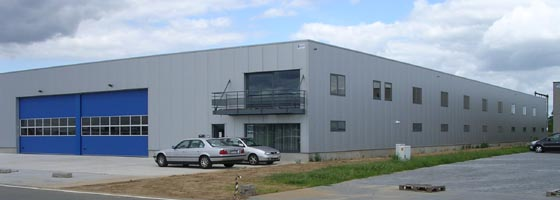
\includegraphics[width=15cm]{pics/PIC001.jpg}
		\caption{Lambert Aircraft Engineering}
		\label{fig:PIC001}
	\end{center}
\end{figure}

The company was created by Filip and Steven LAMBERT in 1996 and is specialized in limited series production of aircrafts and in avionics maintenance. Thanks to the agreements FAA Part 145 and EASA Part M Subpart F, Lambert Aircraft Engineering is authorized to sell and install avionics products on any kind of aircrafts like Dynon, Garmin or Avidyne products.

\bigskip

The avionics workshop sells classic avionics products like headsets, GPS, transponders and so on. It sells pilot accessories, for instance lifejackets, protactors and aeronautical charts. It is also possible to design a new instrument panel for aircrafts and helicopters.

\bigskip

%TODO: diagram of the employees (Manager, 1 design engineer, 1 accountant (secretary?), 3 technicians in mechanical department, 3 in avionics department). PIC002
Decisions are taken quickly and information flows at a fast pace thanks to the simple but effective structure of the team.  There are different nationalities among the staff which demonstrates that the company is very open minded.

\bigskip

Aviation is an international environment. Lambert Aircraft Engineering does business with France, the Netherlands and the United Kingdom. The economy has been very weak since 2009 because of the economy crisis which makes things more difficult. On the aircrafts market the crisis is "noticeable", there a not many aircrafts selled anymore. But for the avionics market, it is still going very well.

\newpage

\subsection{The Mission M108 and the M212}
%photo of the M108 and M212. PIC003
\begin{figure}[ht!]
	\begin{center}
		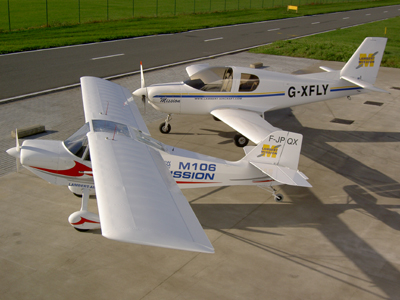
\includegraphics[trim = 0cm 1cm 0cm 1cm,clip]{pics/PIC003.jpg}
		\caption{The Mission M108 and M212}
		\label{fig:PIC003}
	\end{center}
\end{figure}


The M108 is a two seater single engine light sport aircraft with an unswept untapered high wing. It has a welded tubular structure and is provided with the Rotax 912iS engine. The Mission M108 can be customised to meet personal preferences for avionics and instruments. In Europe, it is available as a kit built aircraft.

\bigskip

The M212 is a four seater single engine light aircraft with an unswept untapered high wing. It has a composite airframe.

\subsection{The M108 LSA production}
The Mission M108 is a two seater single engine light sport aircraft. It is in the final stages of development and heading for certification. With the new Rotax 912iS engine installation, the design of every system is carefully reviewed and modified if required. Internal documentation for production, design and avionics departments have to be updated, such as parts lists and 2D production drawings. External documentation provided with the LSA kit to the customer in Europe, for instance the Pilot's Operating Handbook (POH), the Illustrated Parts Catalog (IPC) and the Aircraft Assembly Manual (AAM) are to be completed in parallel with the production of the first M108.

\bigskip

Employees are currently focused on the certification of the Mission M108. Technicians and engineers are working in coordination: when a part is created, the engineer has to draw it and sometimes improve it for better mechanical characteristics. There is no boundary between the production and the design teams as they are working together very closely. I was part of the design team, following the production department in order to be aware of design changes and draw or update new parts for the aicraft.

\newpage

\section{Contribution to the project}
\subsection{CAD and design work}
\subsubsection{Schematics and illustrations}

In order to know better about the functioning of the plane, I was assigned to draw some schematics for the Pilot's Operating Handbook. This manual explains how to maintain the aircraft in case of malfunction. This first job allowed me to get acquainted with AutoCAD and prepare myself for the future designs to come. 

%TODO: pictures of the schematics (fuel system and electrical system) PIC004 PIC005
\begin{figure}[ht!]
	\begin{center}
		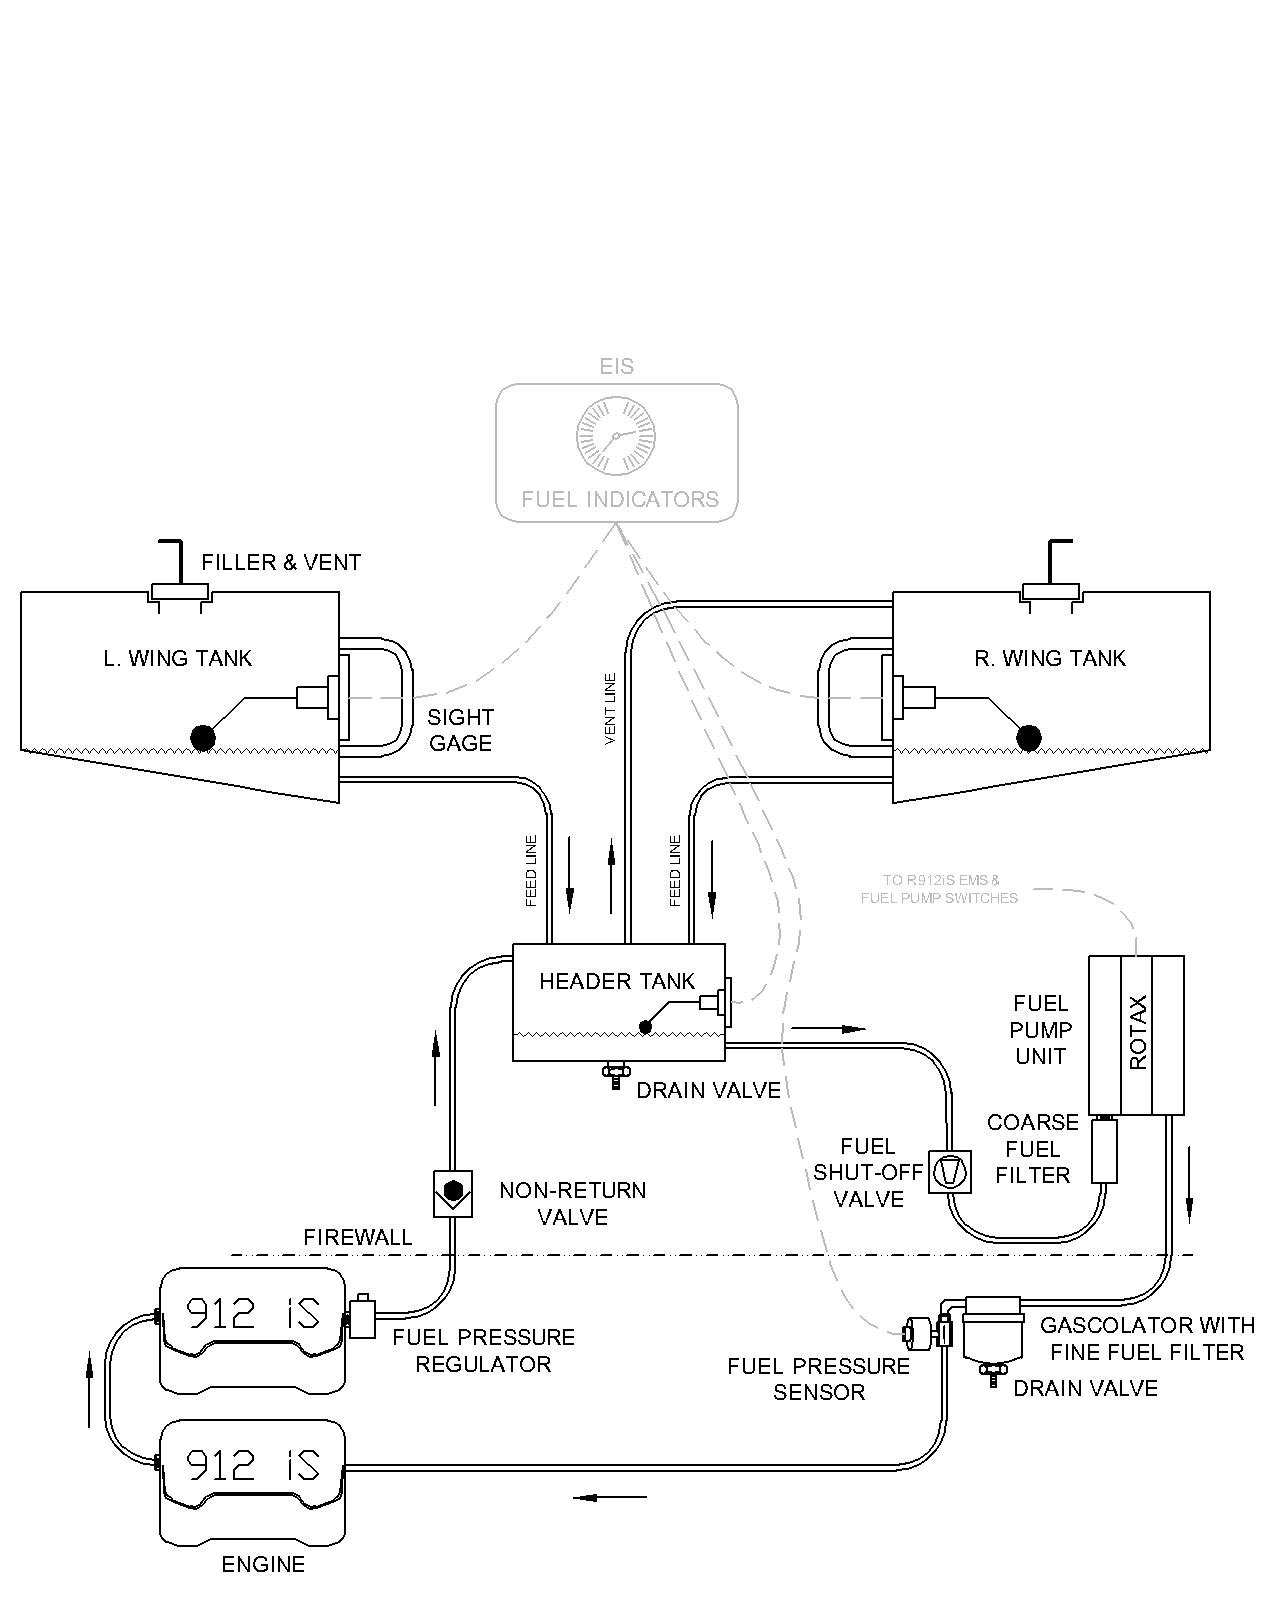
\includegraphics[width=9.5cm, trim = 0.5cm 1cm 0.5cm 12.5cm,clip]{pics/PIC004.jpg}
		\caption{The fuel system of the Mission M108}
		\label{fig:PIC004}
	\end{center}
\end{figure}
\begin{figure}[ht!]
	\begin{center}
		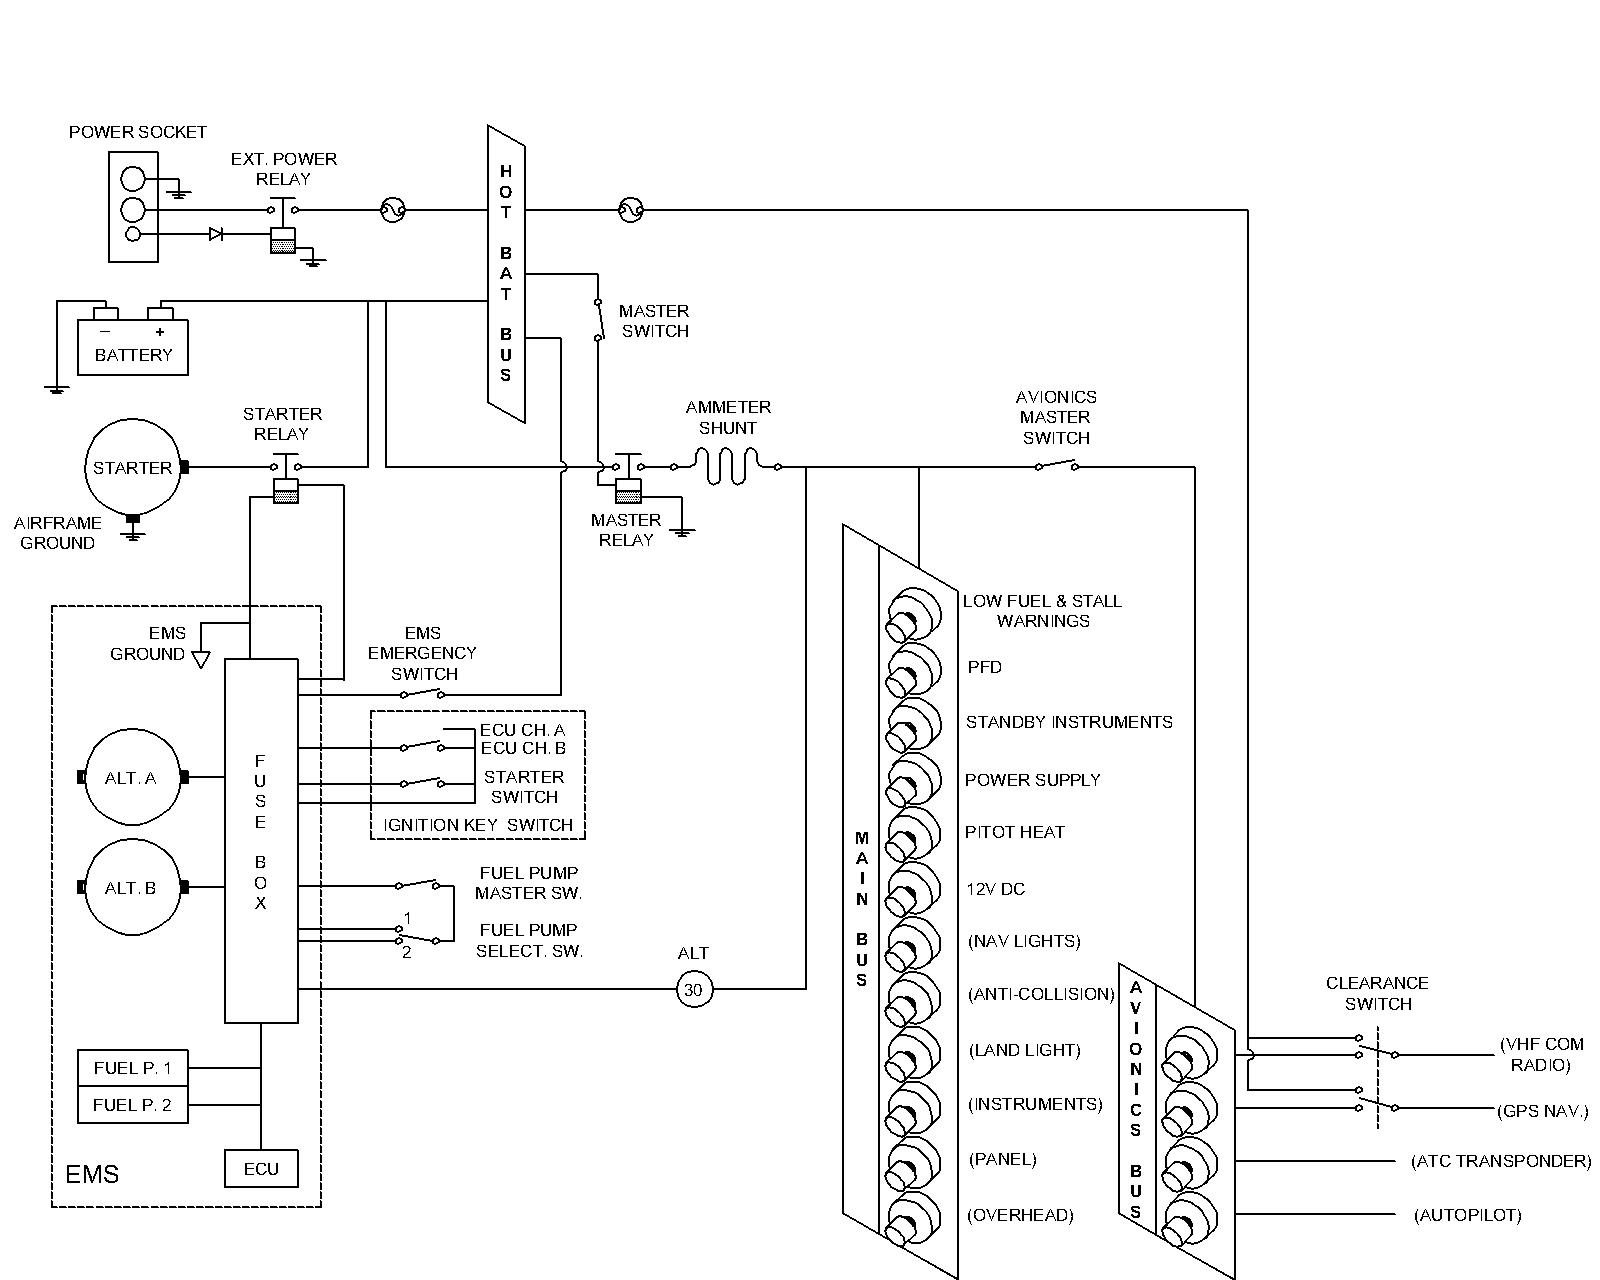
\includegraphics[width=9.5cm, trim = 0.5cm 0cm 0.5cm 2cm,clip]{pics/PIC005.jpg}
		\caption{The electrical system of the Mission M108}
		\label{fig:PIC005}
	\end{center}
\end{figure}

\newpage

I also drew the instrument panel for the Pilot's Operating Handbook to have a global view of the cabin. Depending on the LSTC chosen, we have the instrument panel with the TL instrument or the G3X system.
%TODO: picture of the instrument panel (2D) PIC006
\begin{figure}[ht!]
	\begin{center}
		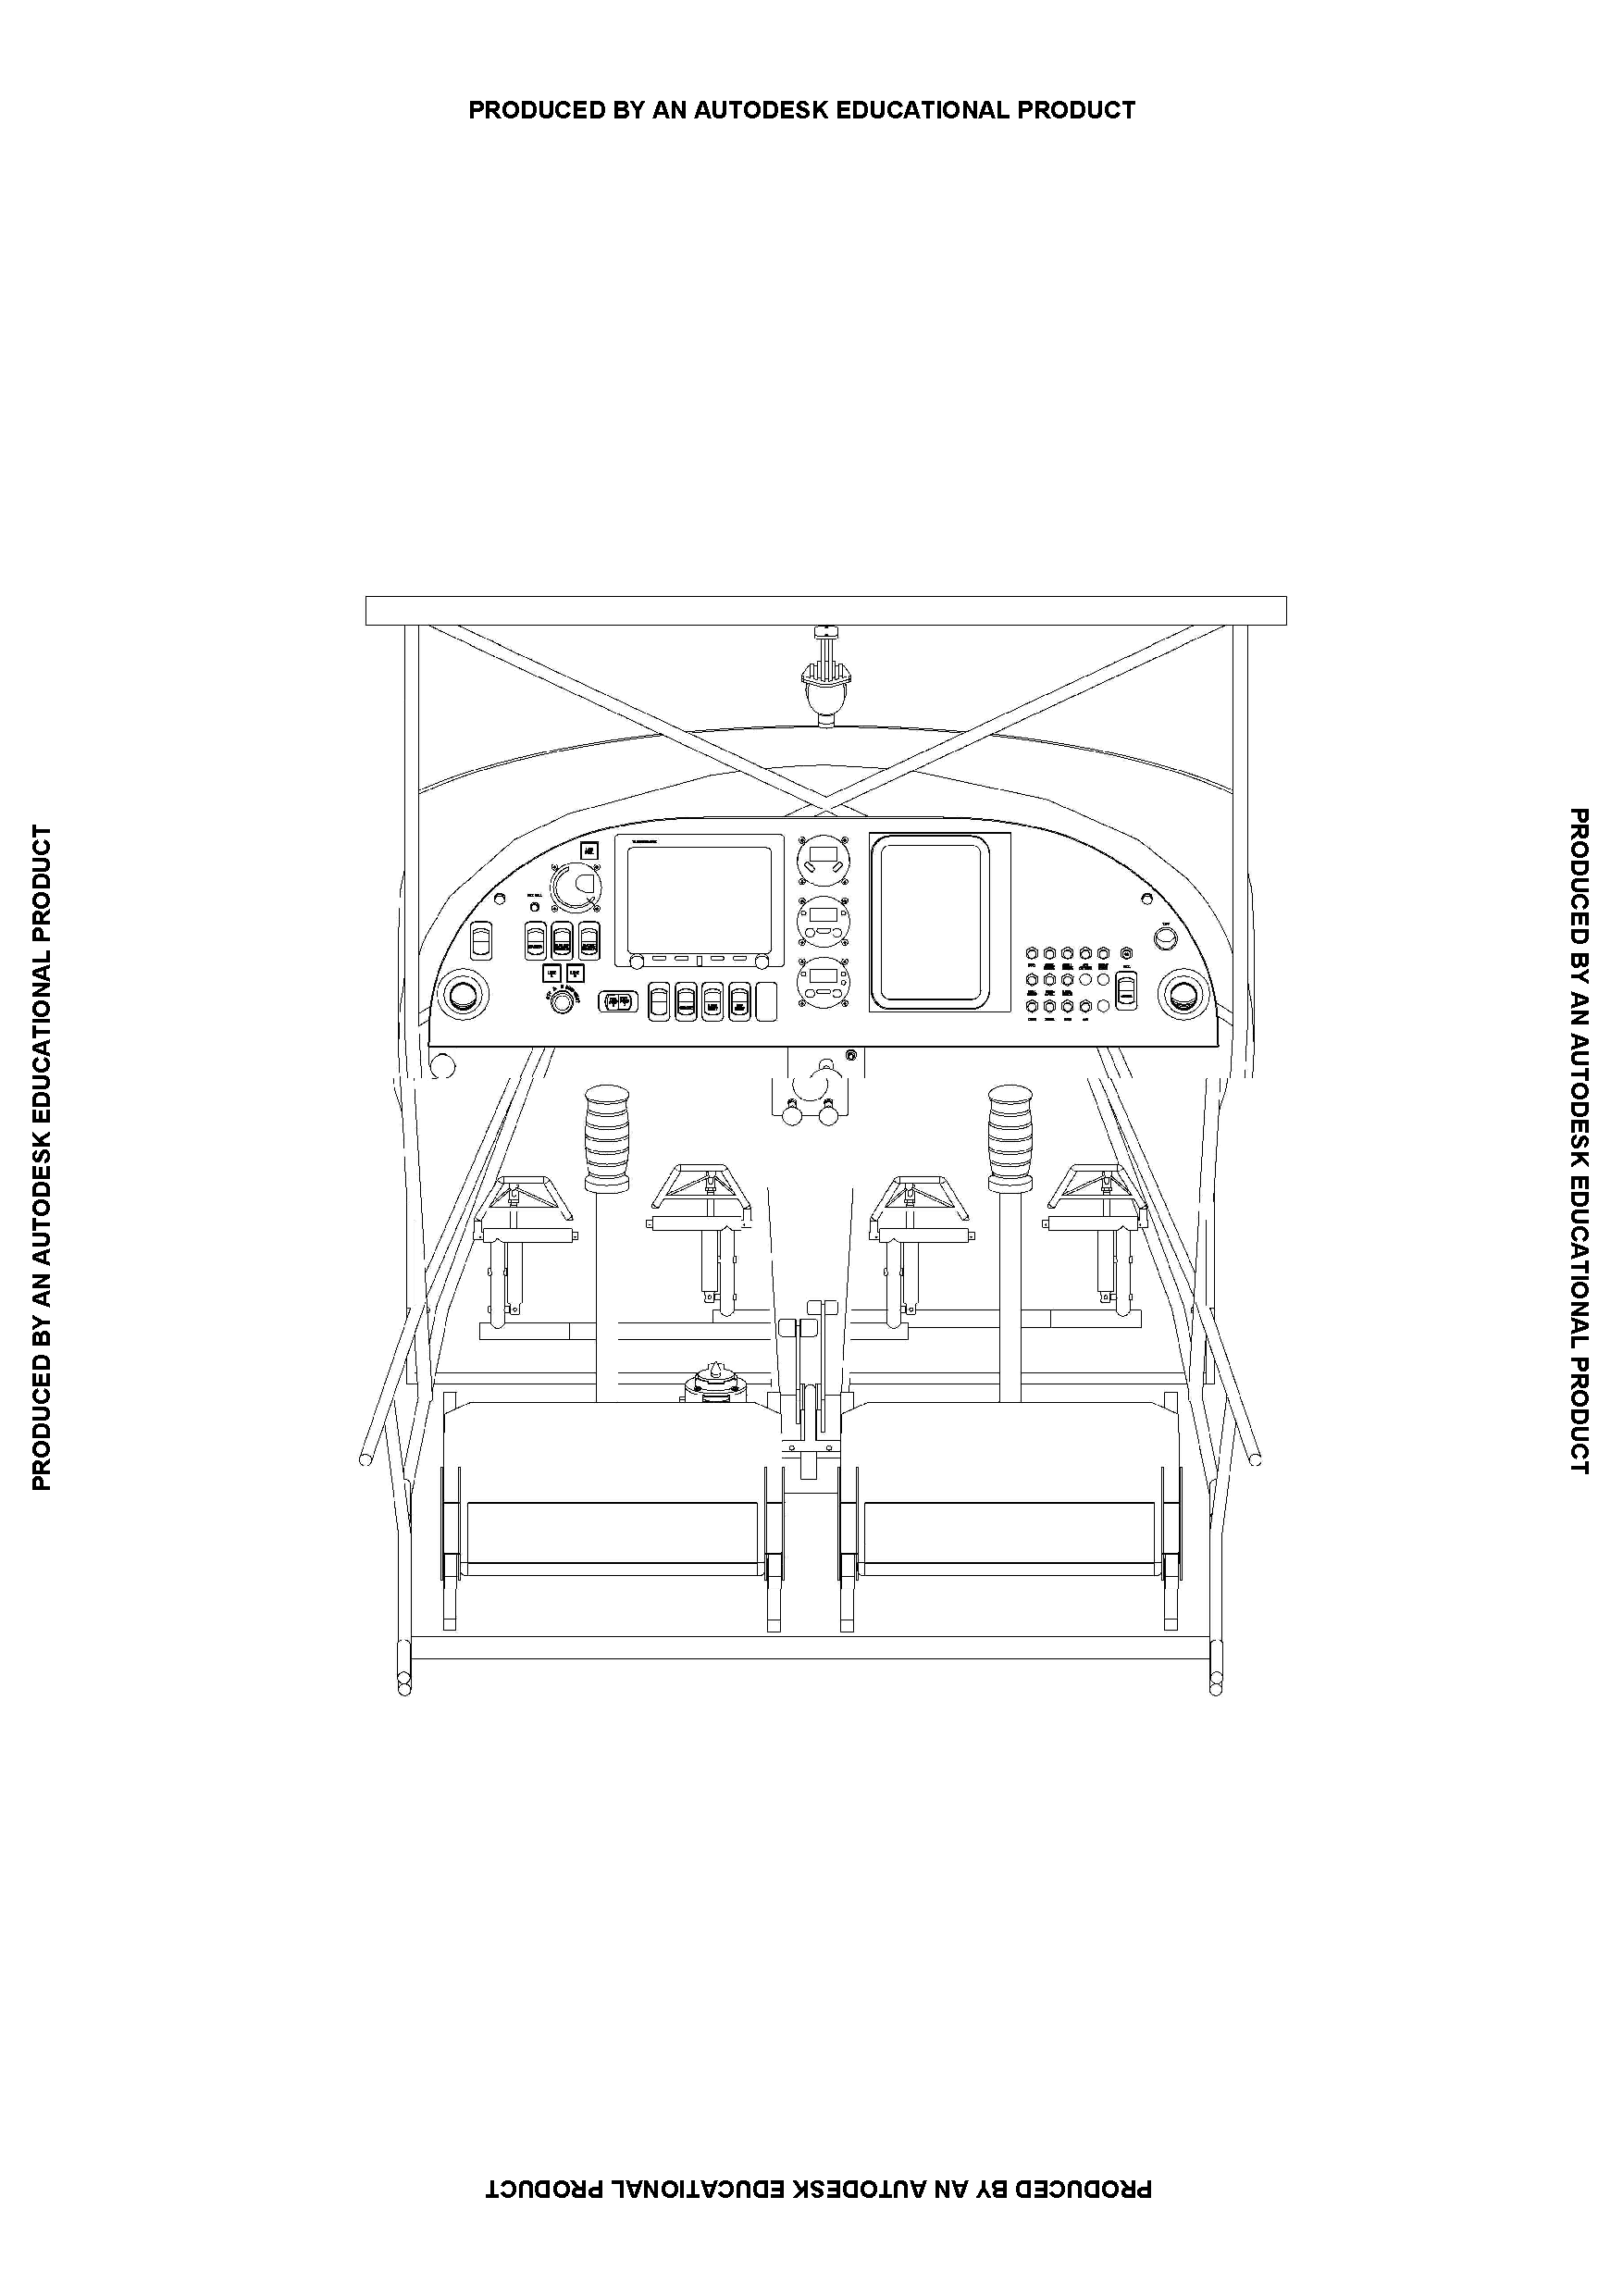
\includegraphics[width=7.5cm,trim = 5cm 10cm 5cm 10cm, clip]{pics/PIC006.pdf}
		\caption{The instrument panel with the TL Elektronic display}
		\label{fig:PIC006}
	\end{center}
\end{figure}

\newpage

\subsubsection{Engine assembly: example of the radiator}

I updated partslists and 2D drawings in case of design modifications, and drew some parts when it was necessary. I will take the example of parts from the radiator and the cabin heating system for explaining my contribution, but I worked on others systems in the meantime.

%TODO: picture of the radiator brackets PIC007
\begin{figure}[ht!]
	\begin{center}
		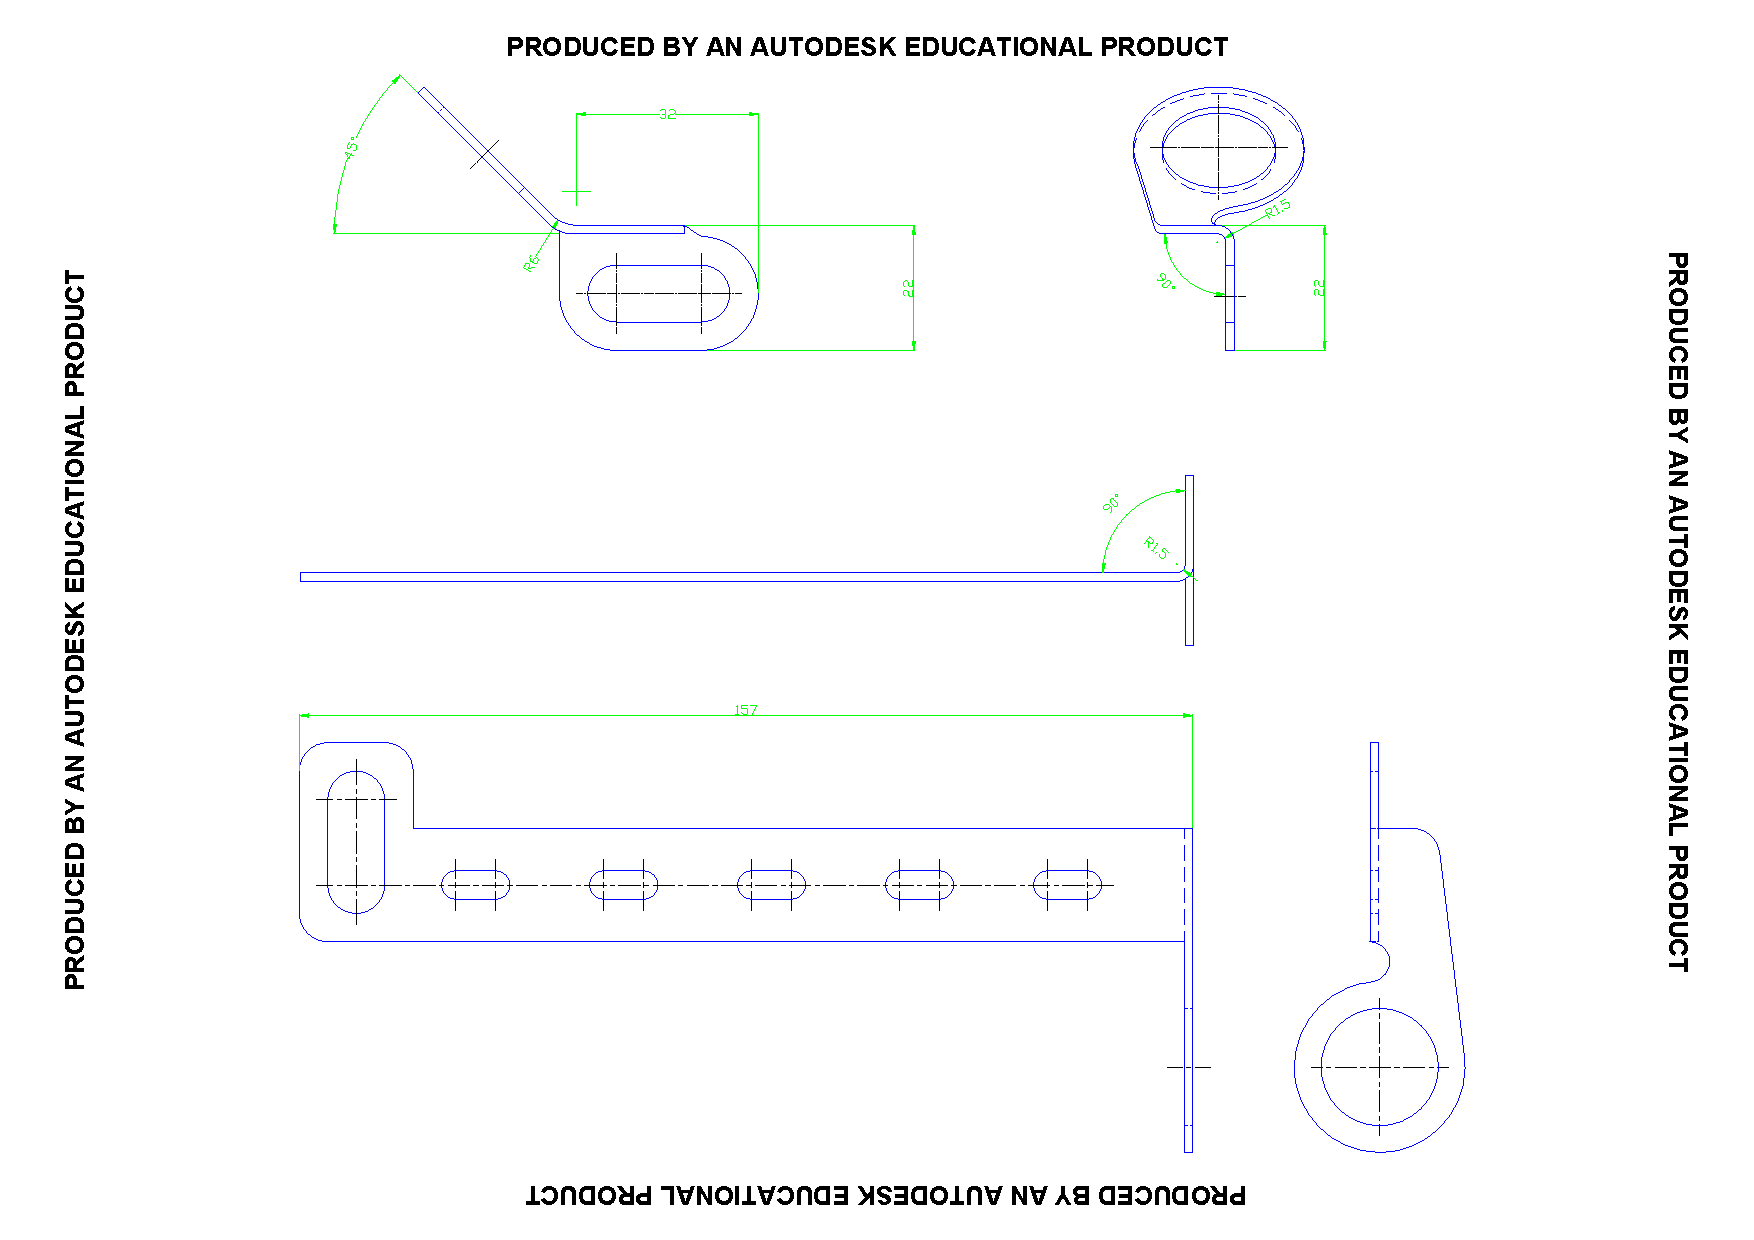
\includegraphics[width=10cm,trim = 2cm 1cm 2cm 1cm, clip]{pics/PIC007.pdf}
		\caption{The upper and lower port side brackets for the radiator}
		\label{fig:PIC007}
	\end{center}
\end{figure}

Designing radiator brackets seemed essential for the Mission M108 because of the original installation. Nothing from our suppliers could match our expectations. We machined the brackets ourselves and bent them for a first try. I drew and improved them in order to be a perfect fit with the baffles.

%TODO: picture of the general assembly of the radiator. PIC008
\begin{figure}[ht!]
	\begin{center}
		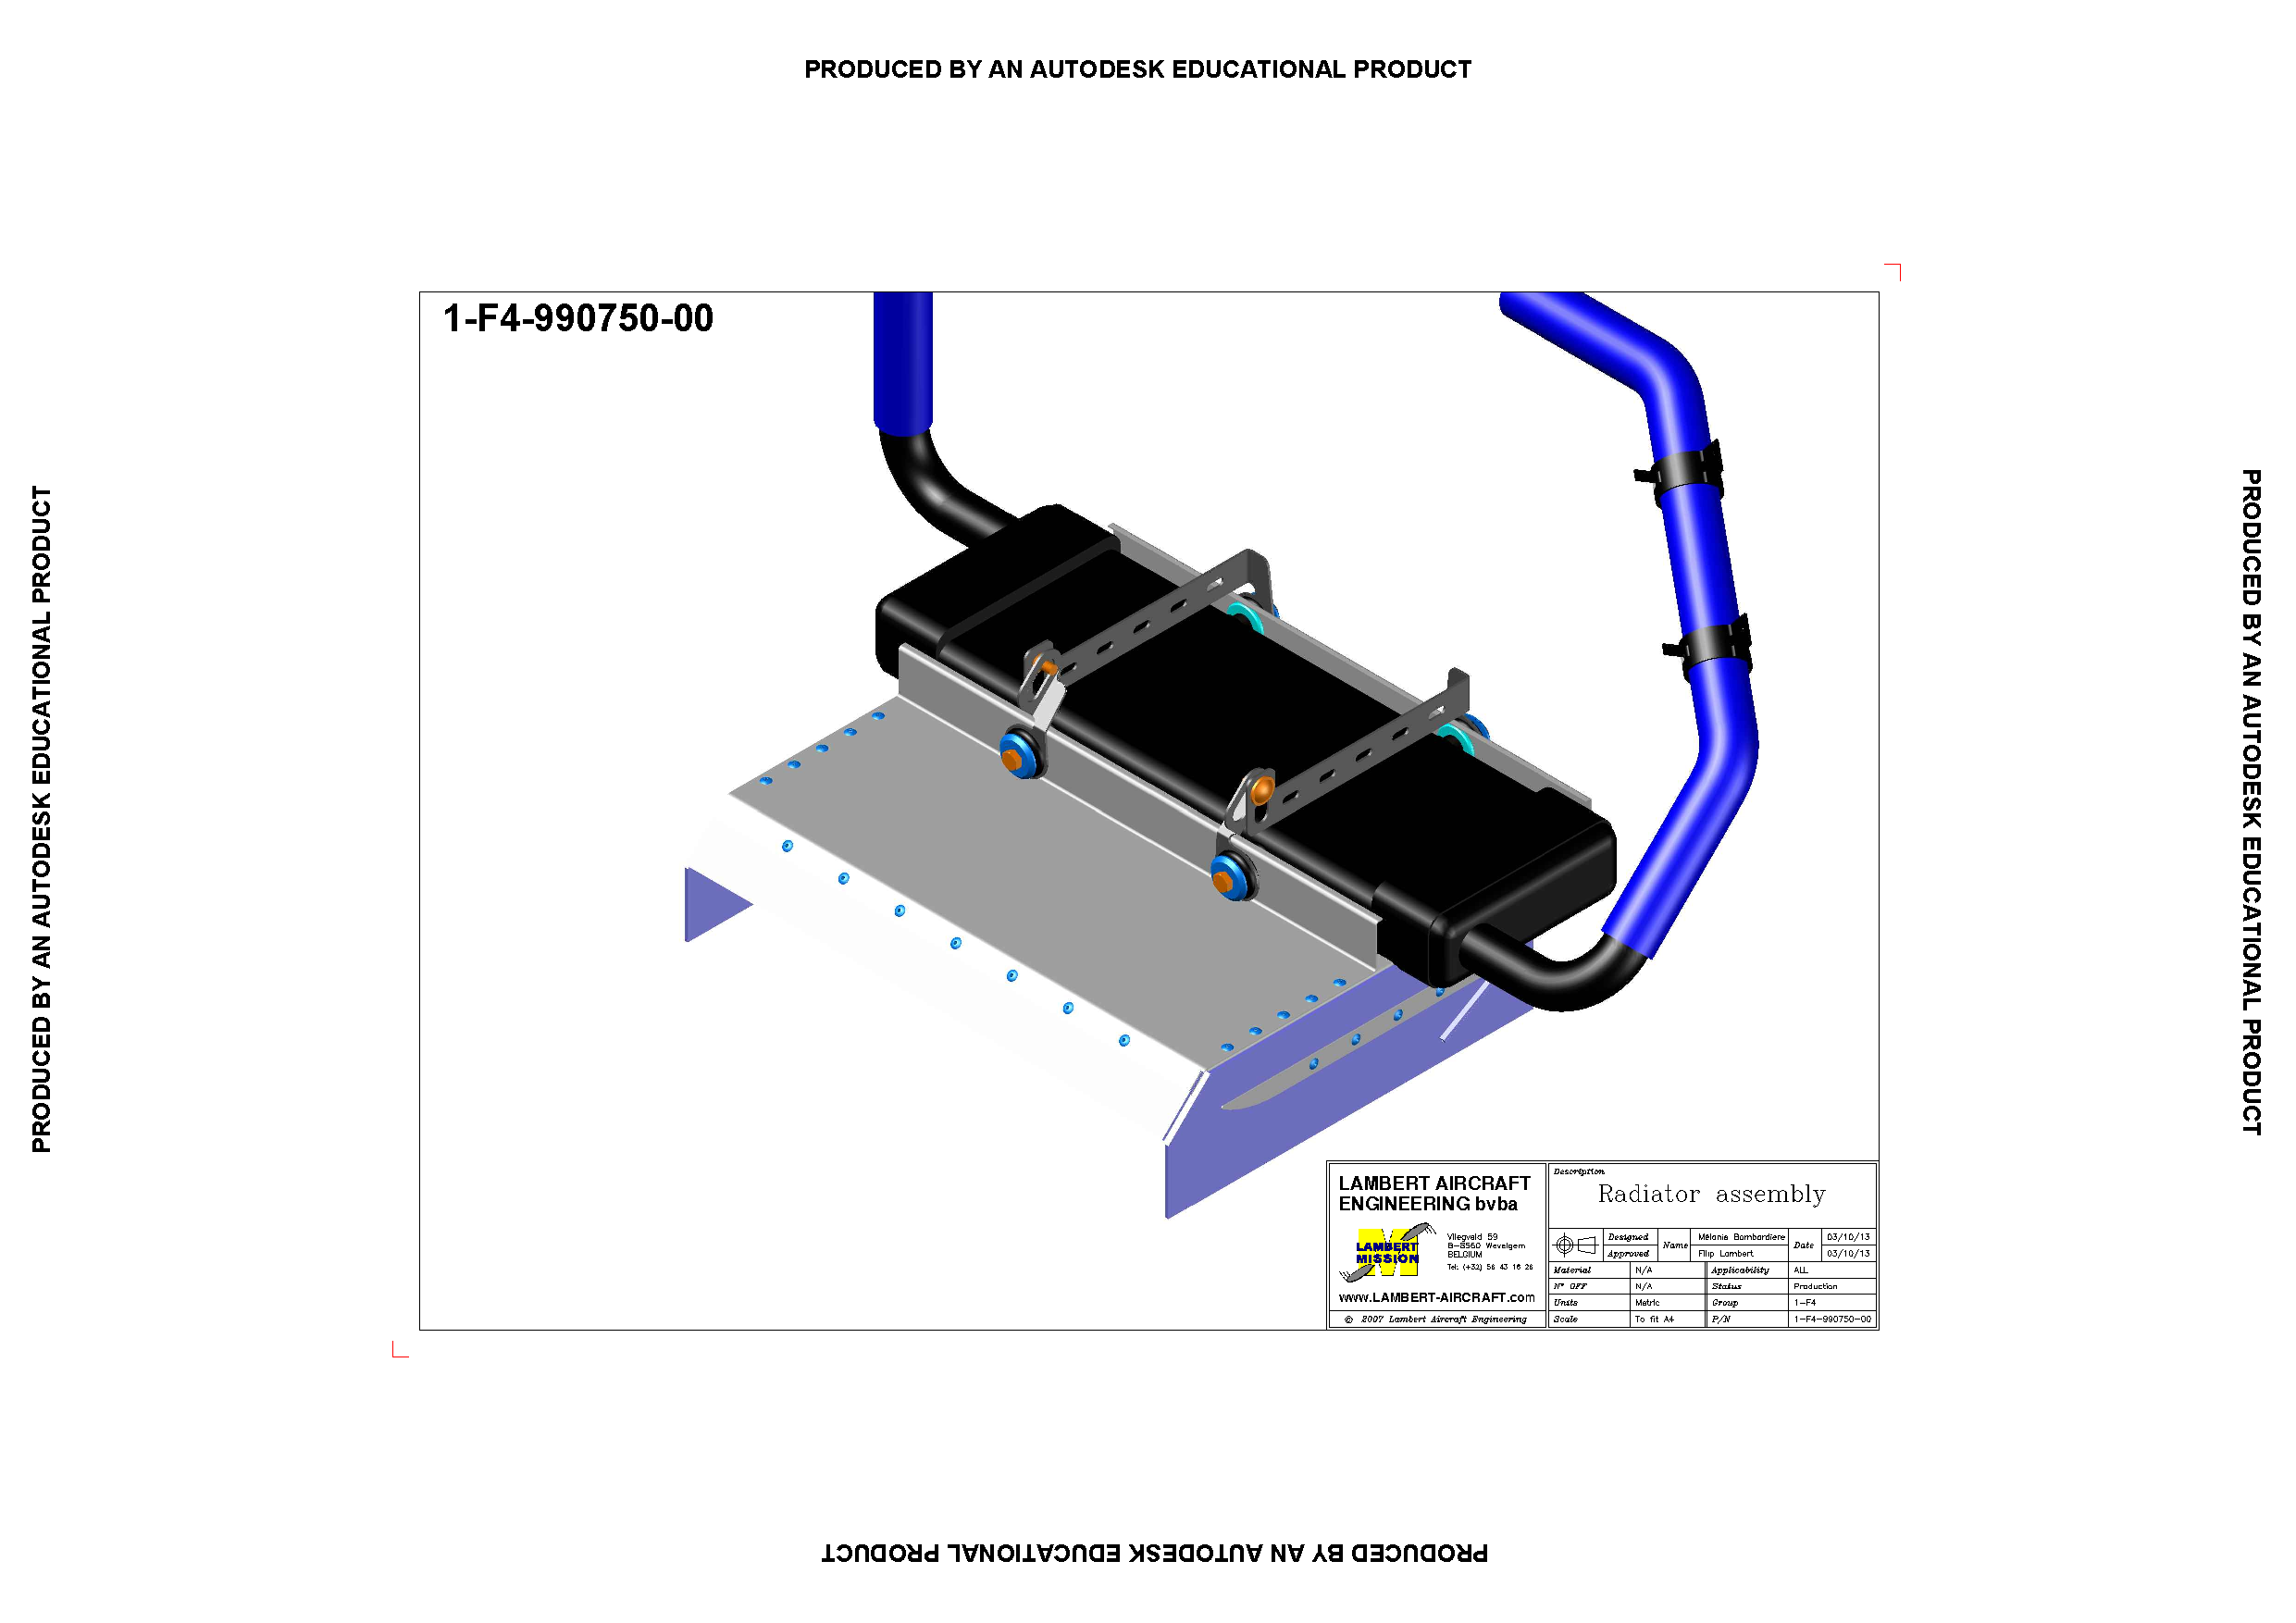
\includegraphics[width=15cm,trim = 5cm 5cm 5cm 5cm, clip]{pics/PIC008.pdf}
		\caption{The radiator assembly}
		\label{fig:PIC008}
	\end{center}
\end{figure}

\newpage

\subsubsection{Cabin heating system: prevention and poka-yoke}

The cabin heating system is an optional feature. It is installed on the firewall, on the engine side. We needed two brackets to mount bowden cables to open or close the valves to heat or not the cabin. These brackets are riveted to the mounting plate and have different lengths. Since we cannot afford to reverse those two, I decided to change the dimensions of the holes for rivets on the brackets and on the mounting plate. This mistake-proofing (poka-yoke) system prevents human errors for an assembly inaccuracy.

%TODO: picture of the two brackets + picture of the assembly PIC009 PIC010
\begin{figure}[ht!]
	\begin{center}
		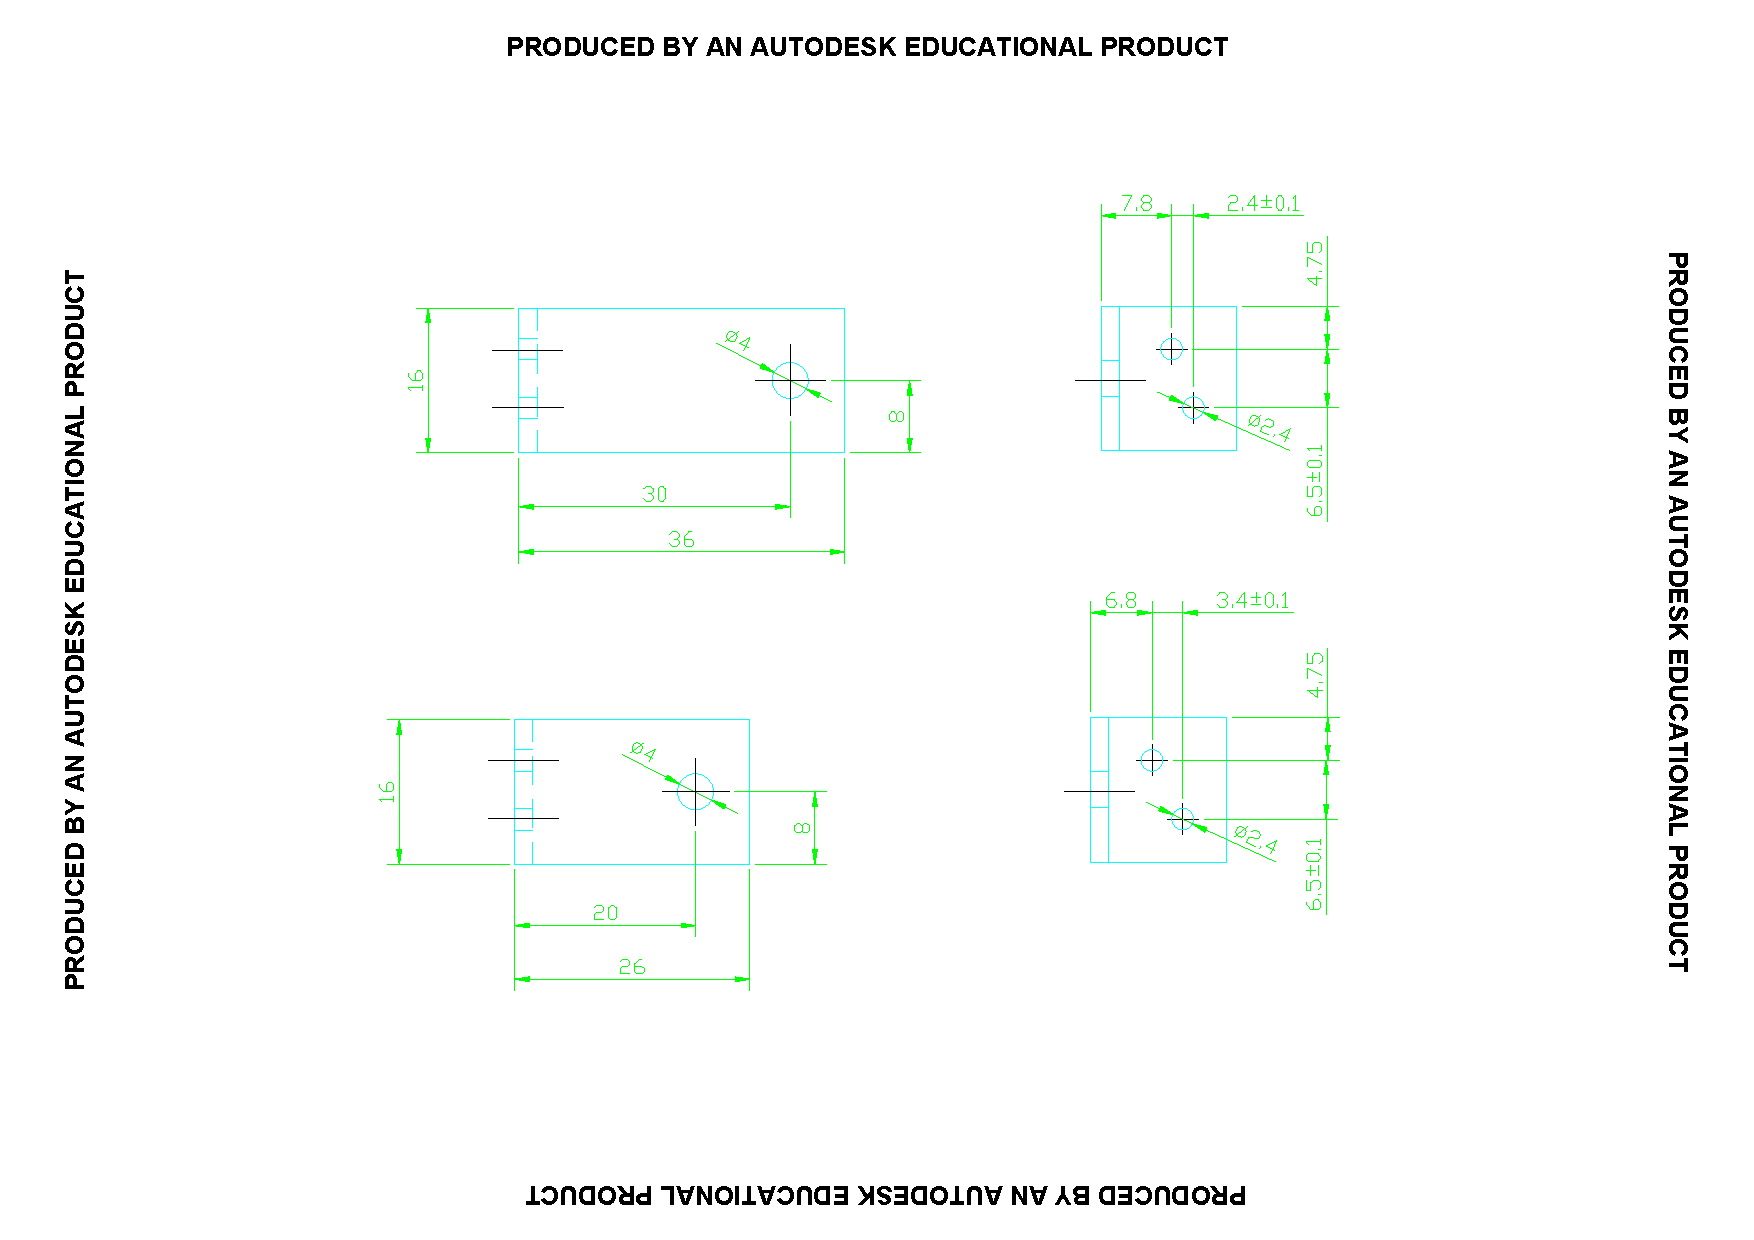
\includegraphics[width=7.5cm,trim = 6cm 4cm 6cm 3cm, clip]{pics/PIC009.pdf}
		\caption{The L-brackets in the cabin heating system}
		\label{fig:PIC009}
	\end{center}
\end{figure}

\newpage

\subsubsection{Illustrated Parts Catalog: combining 3D design and logic}

In parallel with the 2D drawings production, I drew 3D drawings for the Illustrated Parts Catalog (IPC). Since Lambert Aircraft Engineering sells the aircraft as a kit in Europe to homebuilders, they have an IPC in order to explain step by step how to assemble the aircraft correctly with every part referenced.
%TODO: picture of a 3D drawing with an Excel sheet PIC011 PIC012

\newpage

I completed the sections concerning the firewall forward installation, the fuel system and the cabin heating system. I worked first on these sections because I knew how it was working thanks to the schematics. I also had to update sometimes other sections because of design modifications that occurred in the meantime.

%TODO: picture of the F4 and S4 IPC PIC013 PIC014
\begin{figure}[ht!]
	\begin{center}
		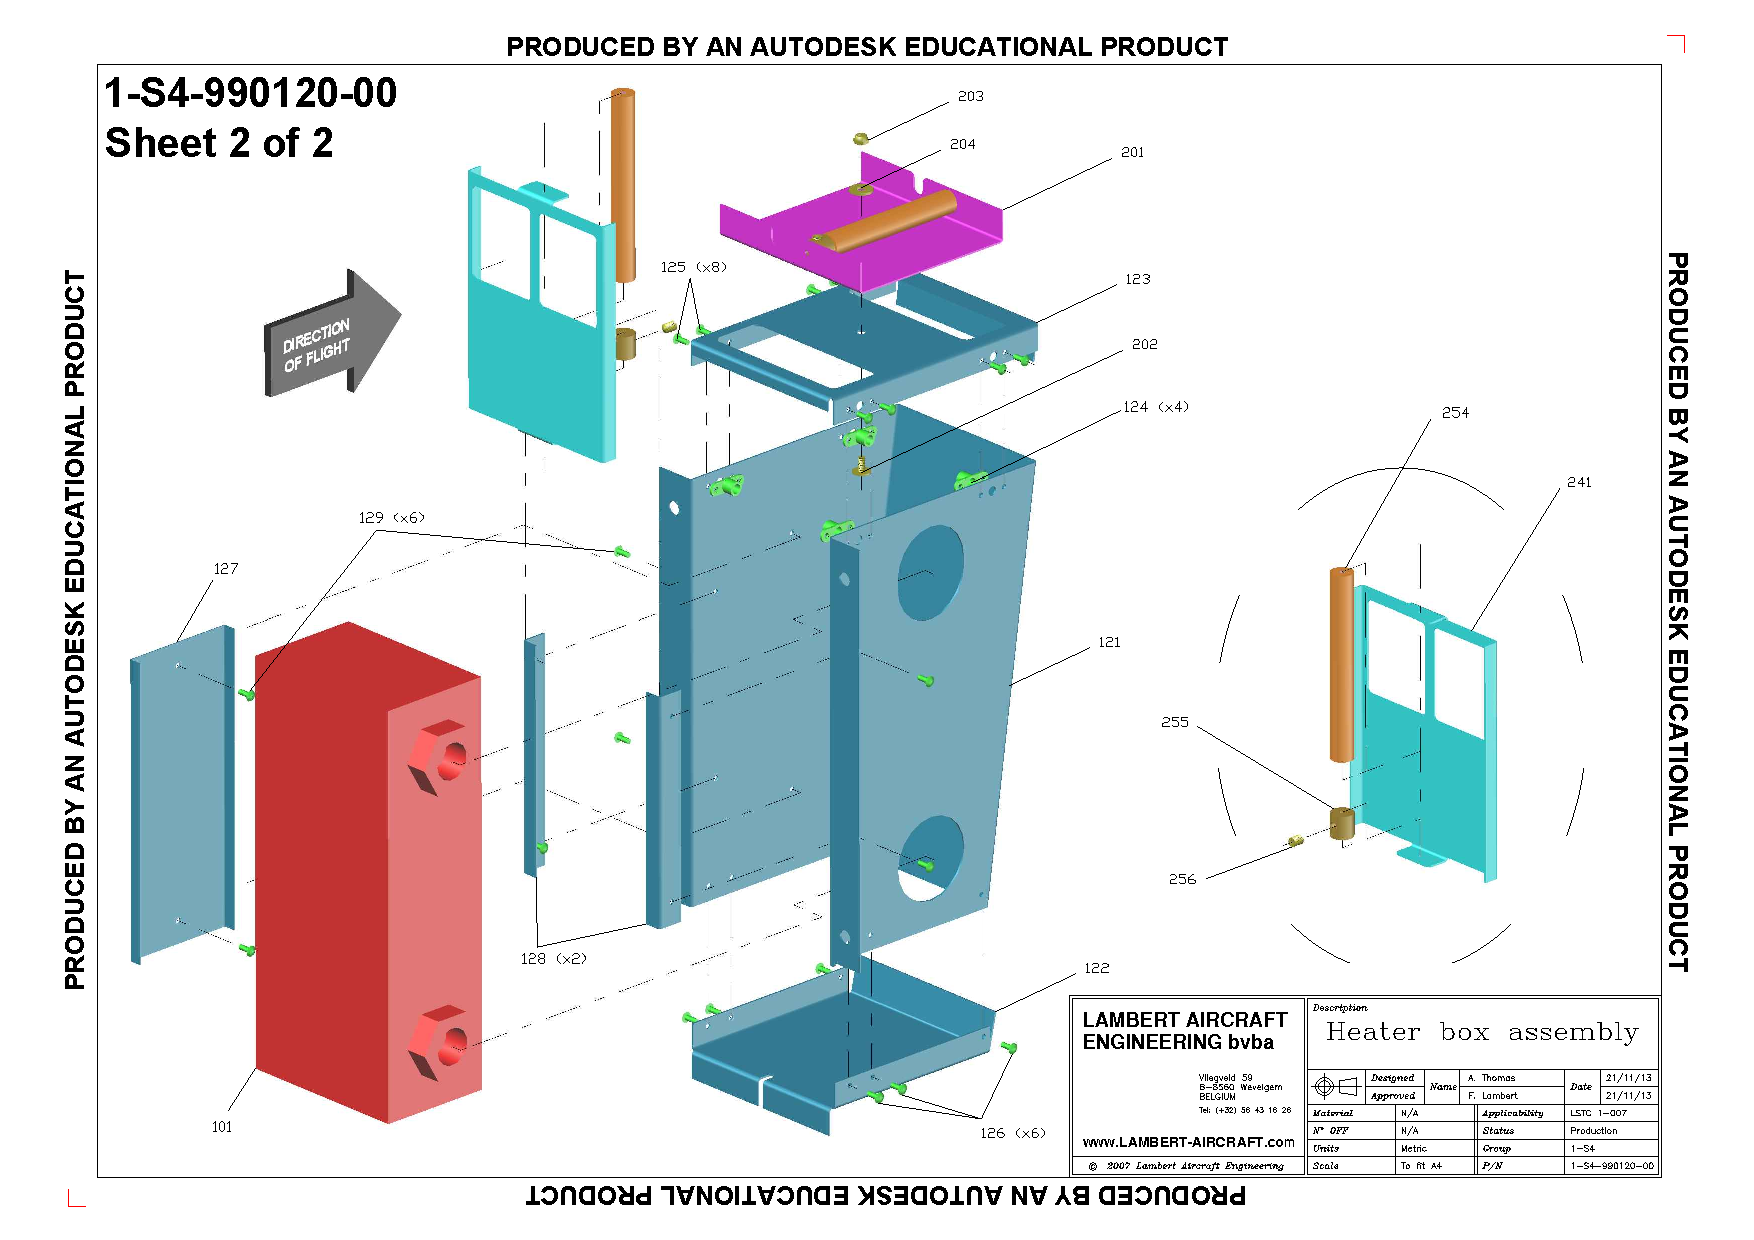
\includegraphics[width=13cm,trim = 1.5cm 1cm 1.5cm 1cm, clip]{pics/PIC013.pdf}
		\caption{The cabin heating system (1-S4)}
		\label{fig:PIC013}
	\end{center}
\end{figure}

\begin{figure}[ht!]
	\begin{center}
		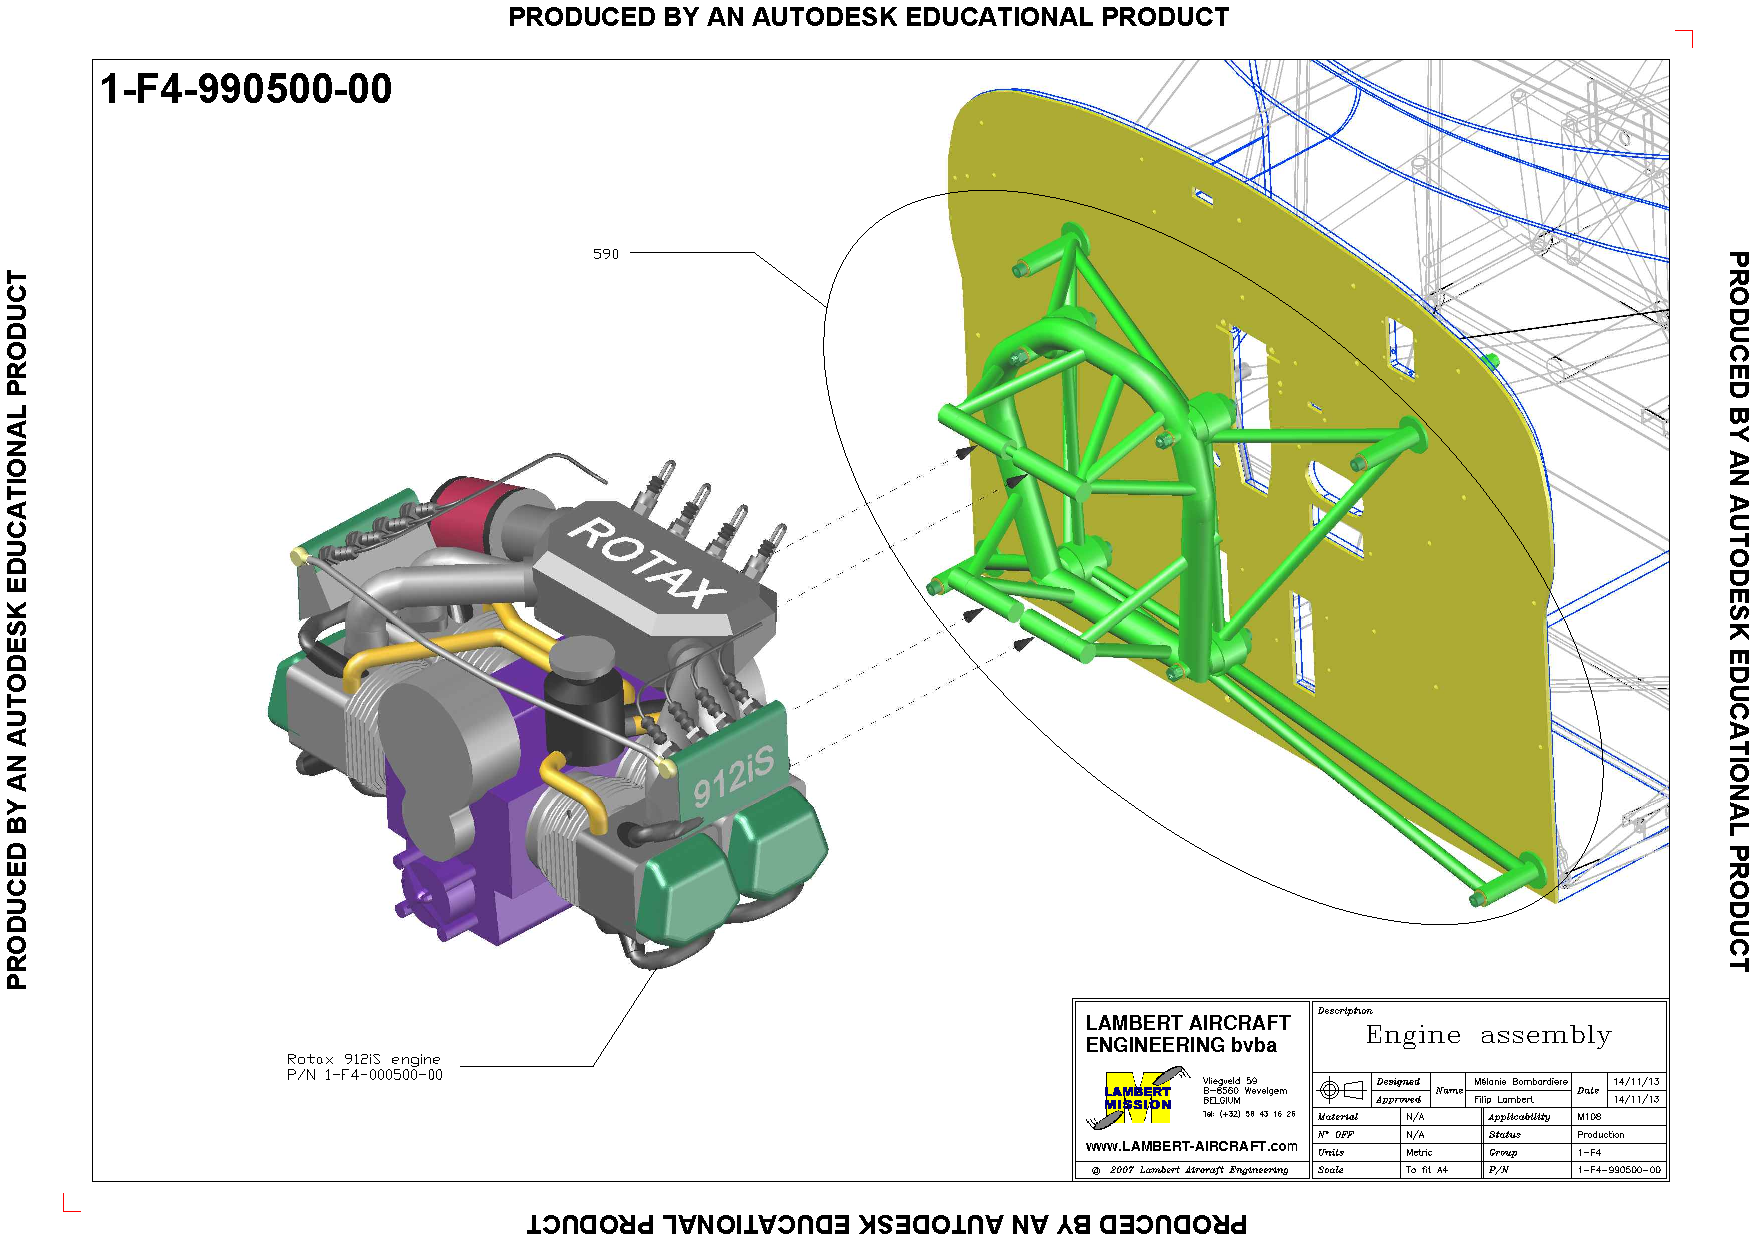
\includegraphics[width=13cm,trim = 1.5cm 0.5cm 1cm 1cm, clip]{pics/PIC014.pdf}
		\caption{The engine installation (1-F4)}
		\label{fig:PIC014}
	\end{center}
\end{figure}

\newpage

I then created all the IPC structure and the 3D drawings for the electrical, Pitot and static, and brake systems. The instrument panel installation is part of the electrical system which includes instruments and avionics equipment.

%TODO: picture of the instrument panel (3D) PIC016
\begin{figure}[ht!]
	\begin{center}
		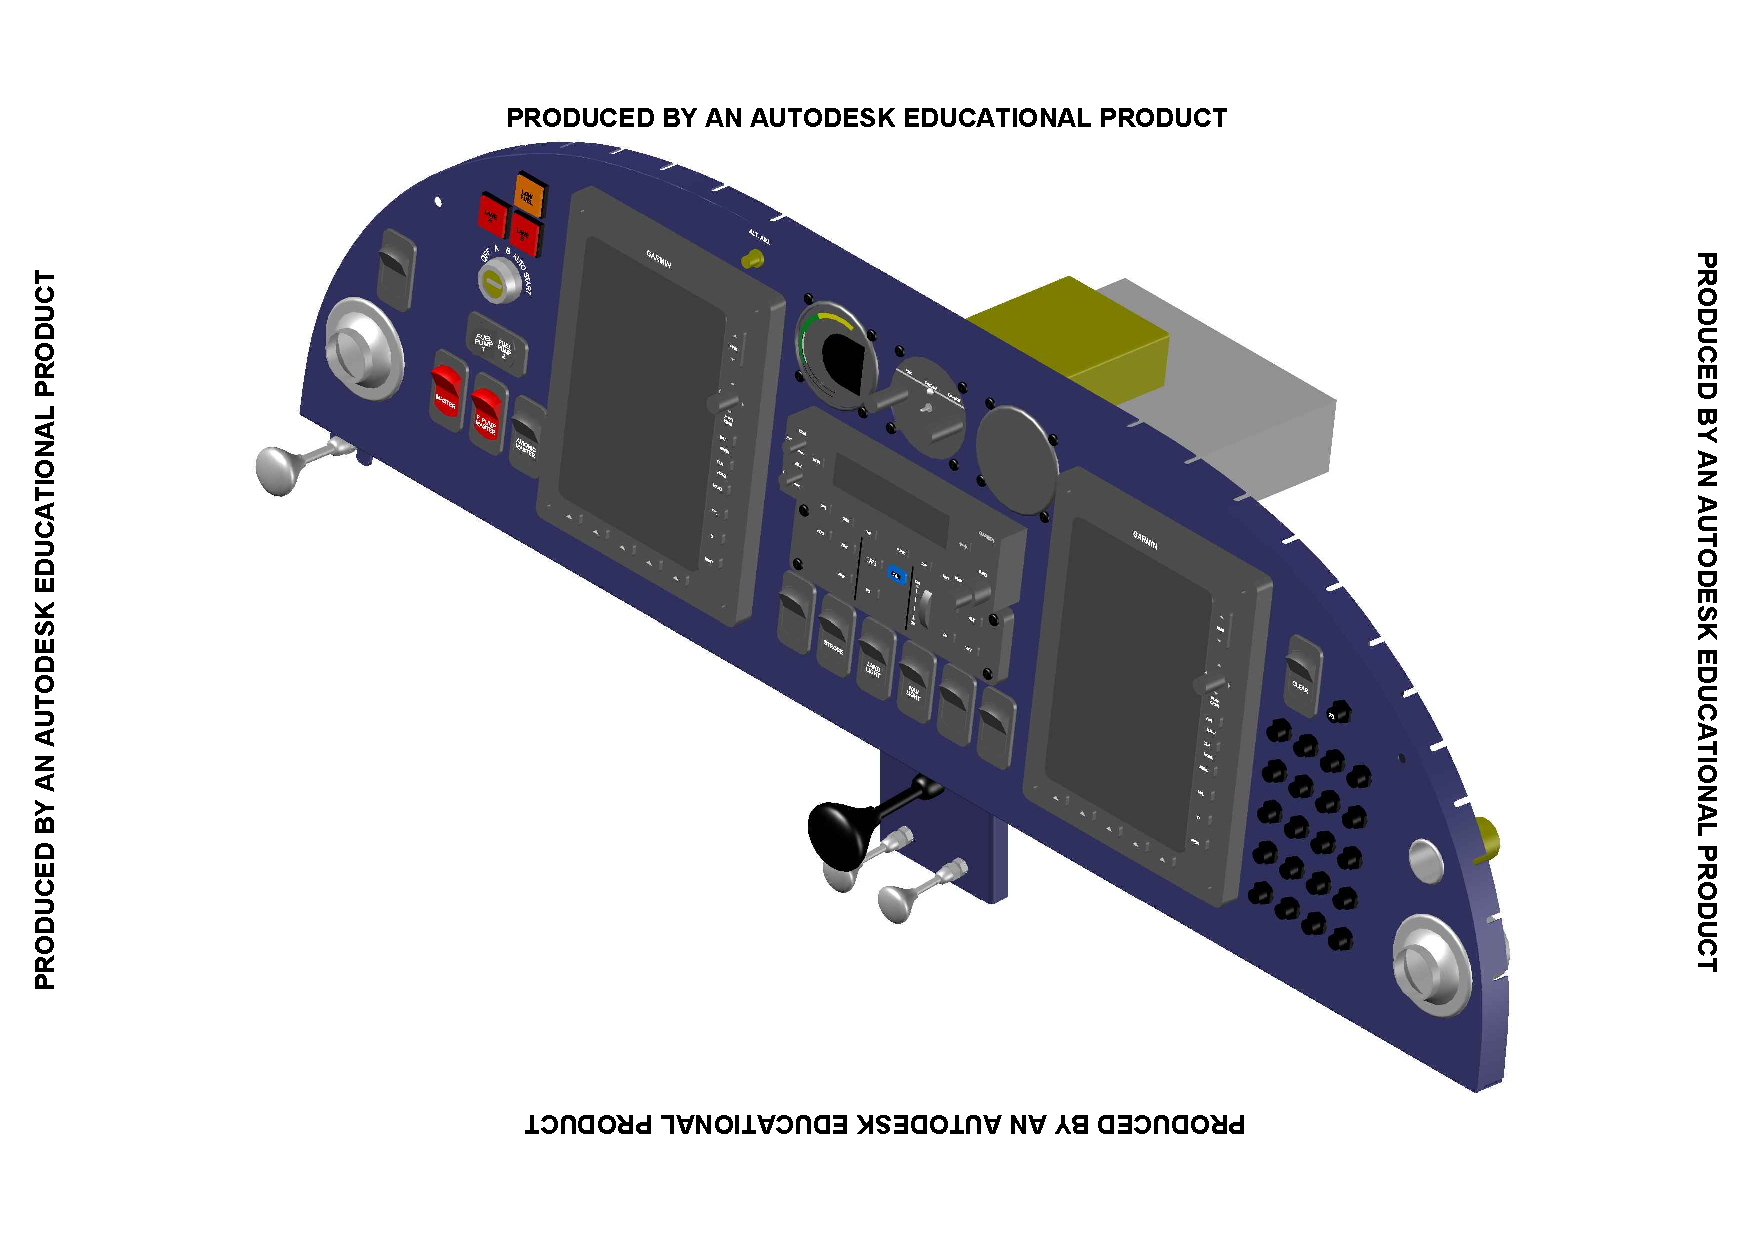
\includegraphics[width=15cm,trim = 2cm 2.2cm 2cm 2.2cm, clip]{pics/PIC016.pdf}
		\caption{The instrument panel}
		\label{fig:PIC016}
	\end{center}
\end{figure}

The electrical system is very complex because it depends on the choice of avionics products the customer wants, and the LSTCs he would like to have. I needed to find a logical structure which can group the common equipment, and separate every option to keep it as simple as possible.

\bigskip

This structure takes into account the basic electrical components which are present anyway, and each option is defined with one part number. If the client needs to see how to install the navigation lights, he will need to reach the 1-S2-995300-00 drawing for further information.

%TODO: picture of the 1-S2 IPC structure PIC015
%refer to the structure later
\begin{figure}[ht!]
	\begin{center}
		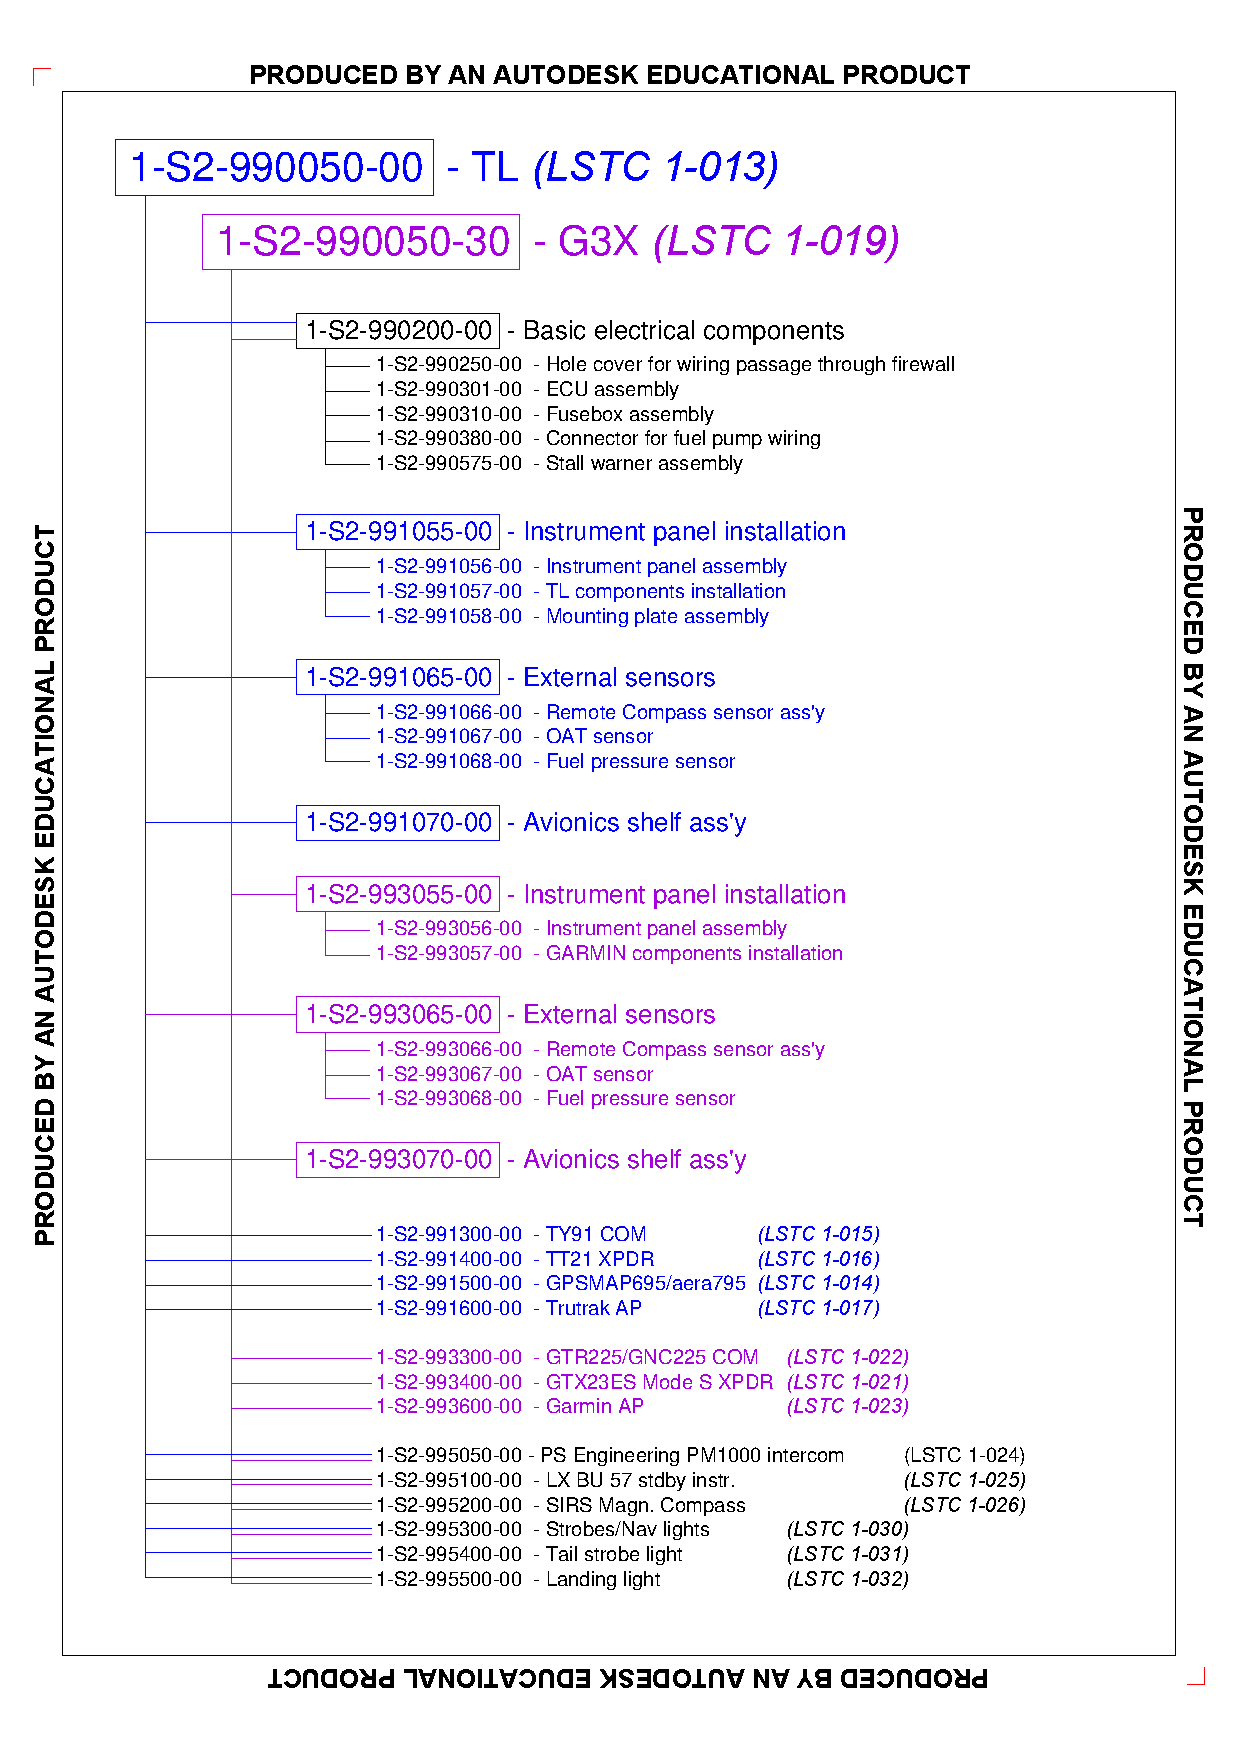
\includegraphics[width=15cm,trim = 1.9cm 2.4cm 1.9cm 2.4cm, clip]{pics/PIC015.pdf}
		\caption{The IPC structure for the electrical system}
		\label{fig:PIC015}
	\end{center}
\end{figure}

\newpage

\subsubsection{Pitot \& static and brake installations: rethinking existing systems}

The Pitot and static systems are not new, but there was no parts list and assembly drawings for that. According with the production, I created the parts list in coordination with the previous installations.

\bigskip

A new Pitot probe is used with the Garmin avionics. It is a heated Pitot probe which requires a heater installed in the wing. Some design work still needs to be done: accessibility to the heater is necessary in case of failures and the team is working on it.

\bigskip

%TODO: picture of the 1-S5 IPC PIC017
\begin{figure}[ht!]
	\begin{center}
		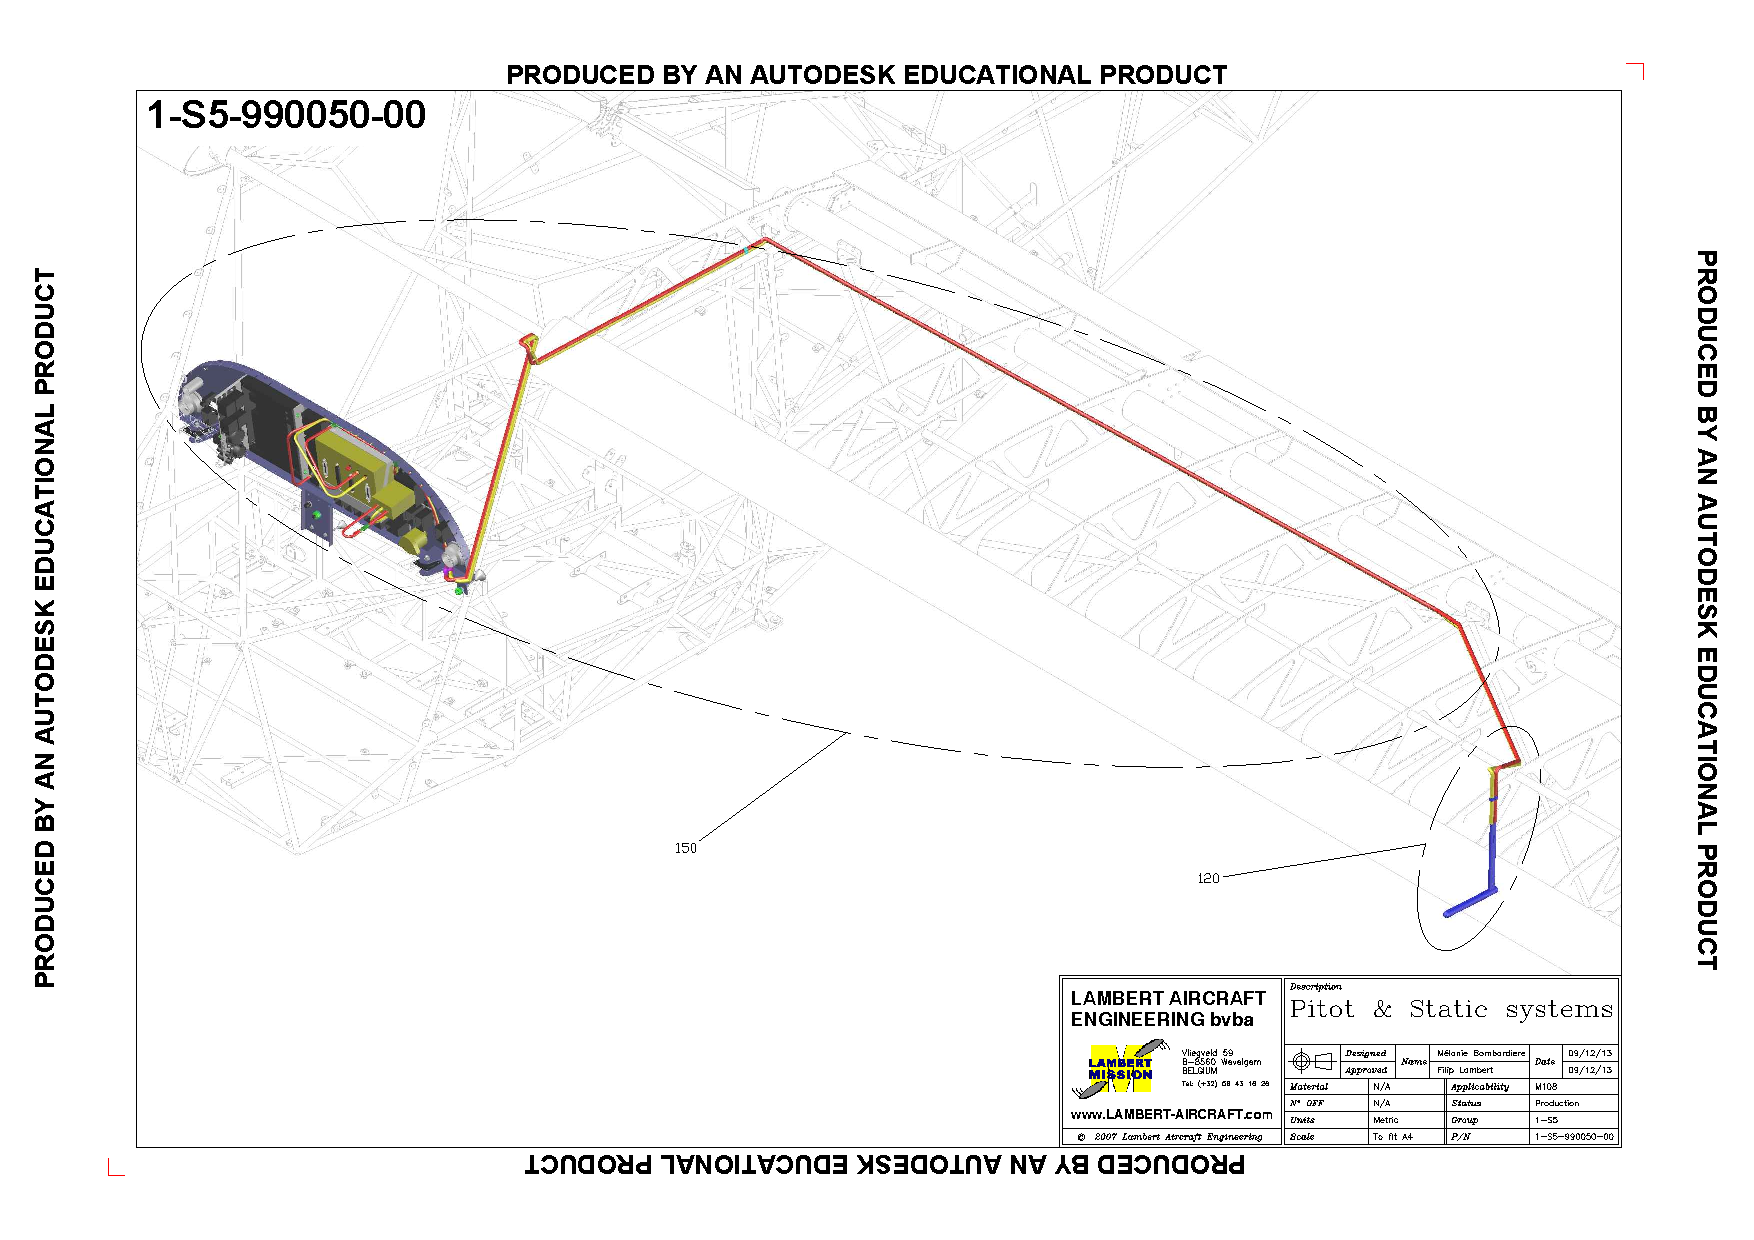
\includegraphics[width=15cm,trim = 1.5cm 1.5cm 1.5cm 1.5cm, clip]{pics/PIC017.pdf}
		\caption{The Pitot and static system (1-S5)}
		\label{fig:PIC017}
	\end{center}
\end{figure}

\newpage

The brake system was an important part of the internship. The 2D and 3D drawings already existed but for the tailwheel version.
%TODO: add an explanation in the glossary for the tailwheel and nosewheel version

\bigskip

In coordination with the design and the production teams, we designed the new brake system but for a nosewheel version. This was totally provisional and the design work has been done at the same time as the installation.

%TODO: picture of the 1-S6 IPC (0051-00) PIC019
\begin{figure}[ht!]
	\begin{center}
		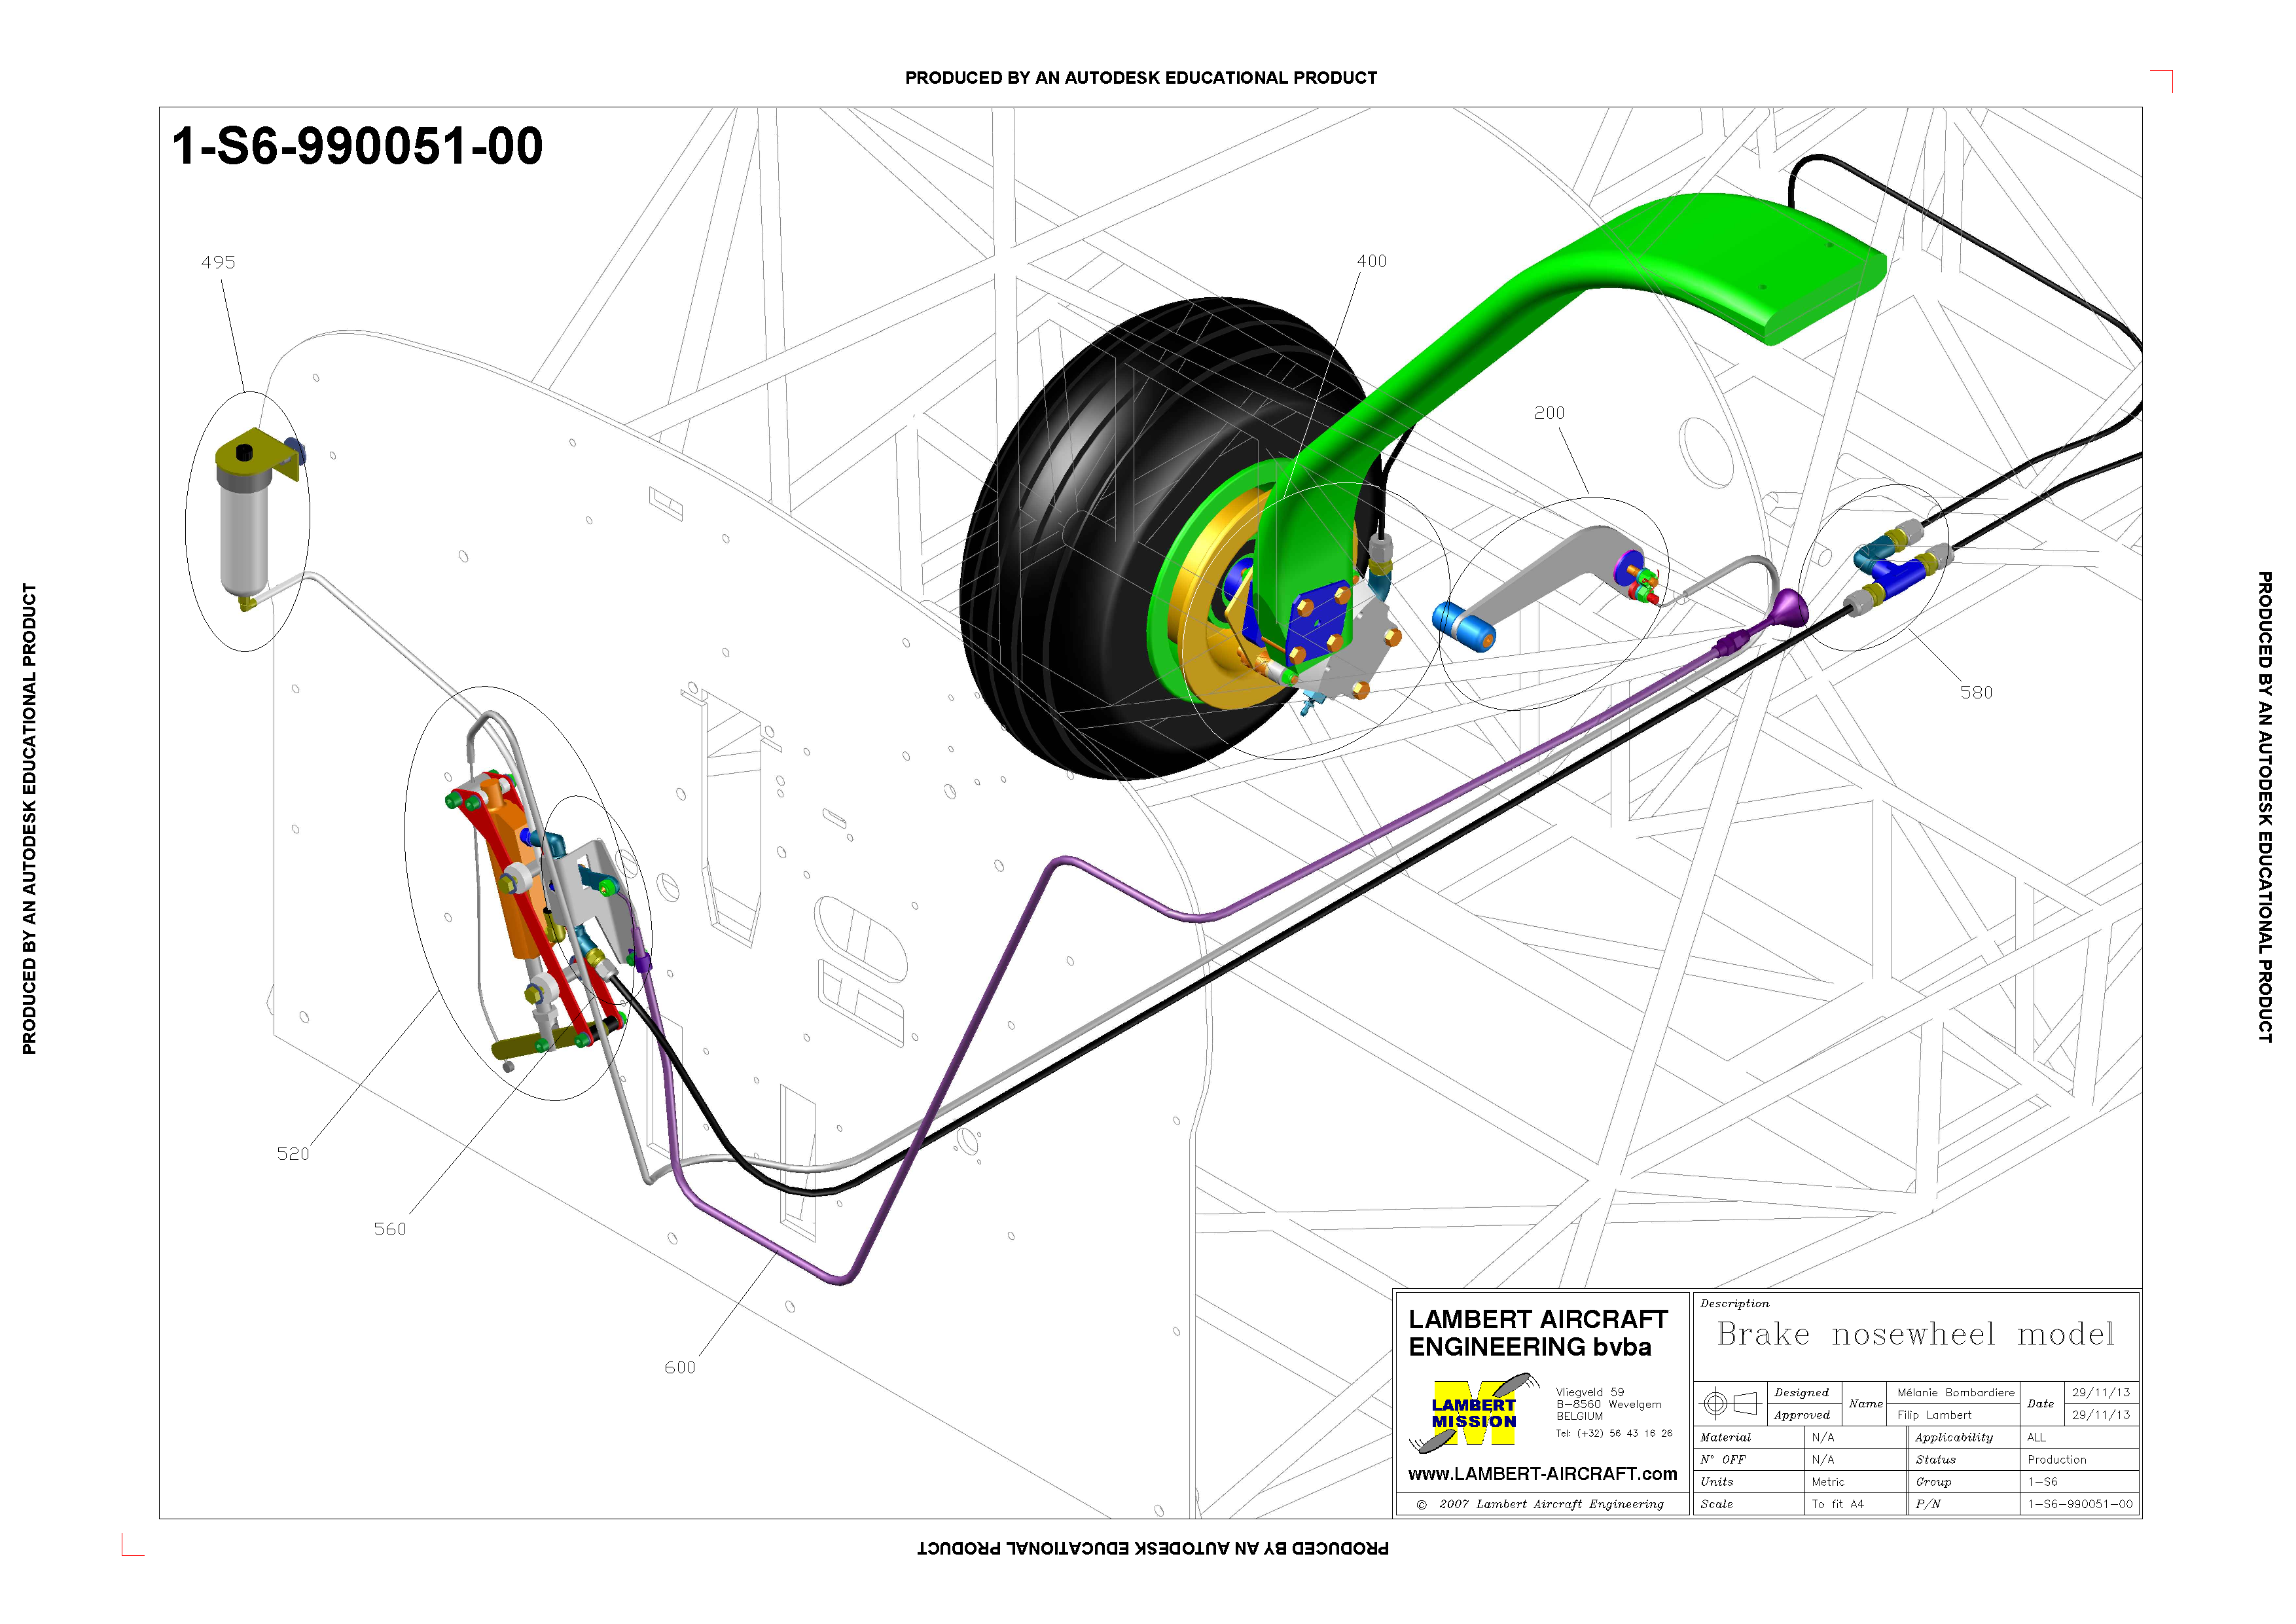
\includegraphics[width=15cm,trim = 1.5cm 2.5cm 1.5cm 2.5cm, clip]{pics/PIC019.pdf}
		\caption{The brake system}
		\label{fig:PIC019}
	\end{center}
\end{figure}

We also thought that the splitter should have been installed directly in the outlet of the master brake cylinder. Indeed, the price of hydraulic lines depends nore on the quantity than the length. This design change can save one hydraulic line, approximately 50 euros. The first M108 will be provided with the first version of the brakes but the next will have the splitter installed on the master brake cylinder.
%TODO: picture of the splitter PIC020
\begin{figure}[ht!]
	\begin{center}
		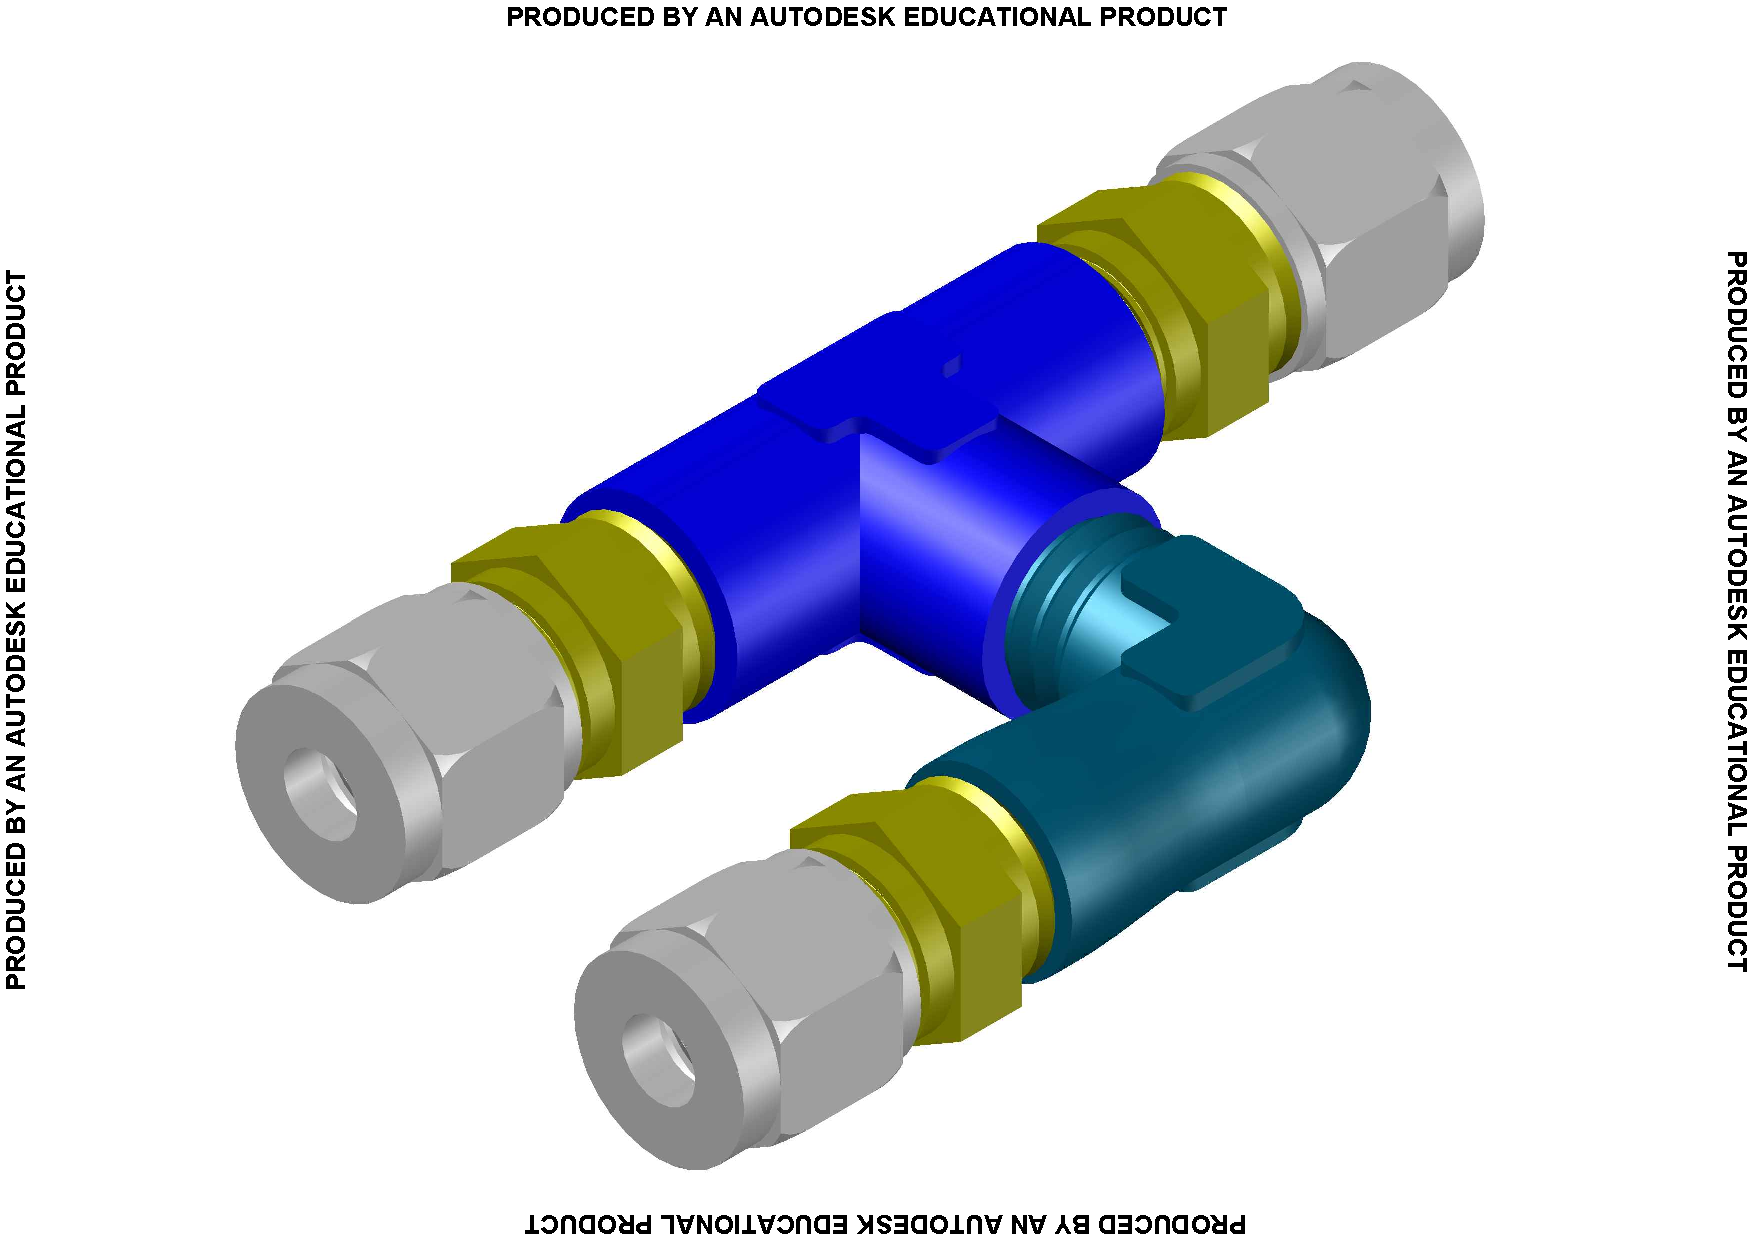
\includegraphics[width=5cm,trim = 1cm 1cm 1cm 1cm, clip]{pics/PIC020.pdf}
		\caption{The splitter}
		\label{fig:PIC020}
	\end{center}
\end{figure}

\newpage

%TODO: picture of the previous position of the spliiter PIC021
%TODO: picture of the new position of the splitter PIC022
\begin{figure}[ht!]
	\begin{center}
		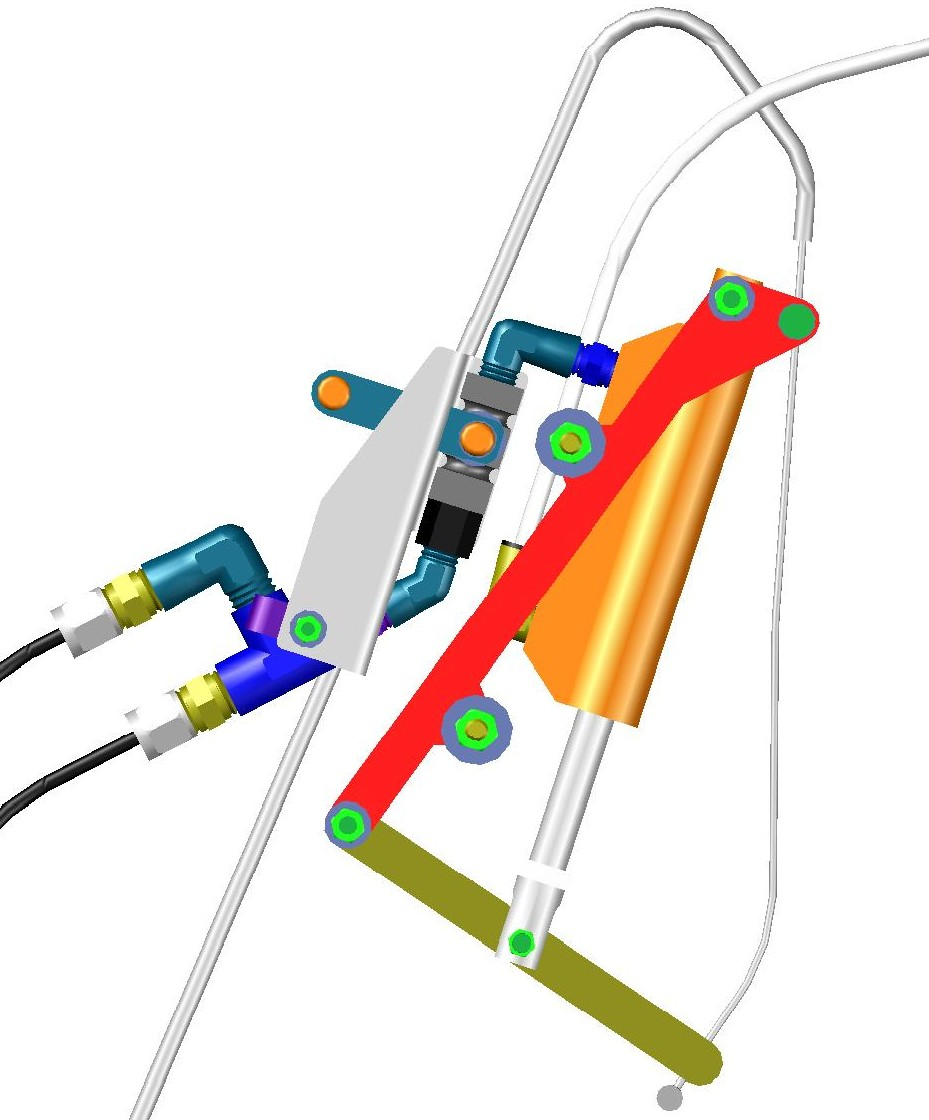
\includegraphics[width=7.5cm]{pics/PIC022.jpg}
		\caption{The new position of the splitter in the brake assembly}
		\label{fig:PIC022}
	\end{center}
\end{figure}

\bigskip

%TODO: picture of the 1-S6 IPC (0051-01) PIC023
\begin{figure}[ht!]
	\begin{center}
		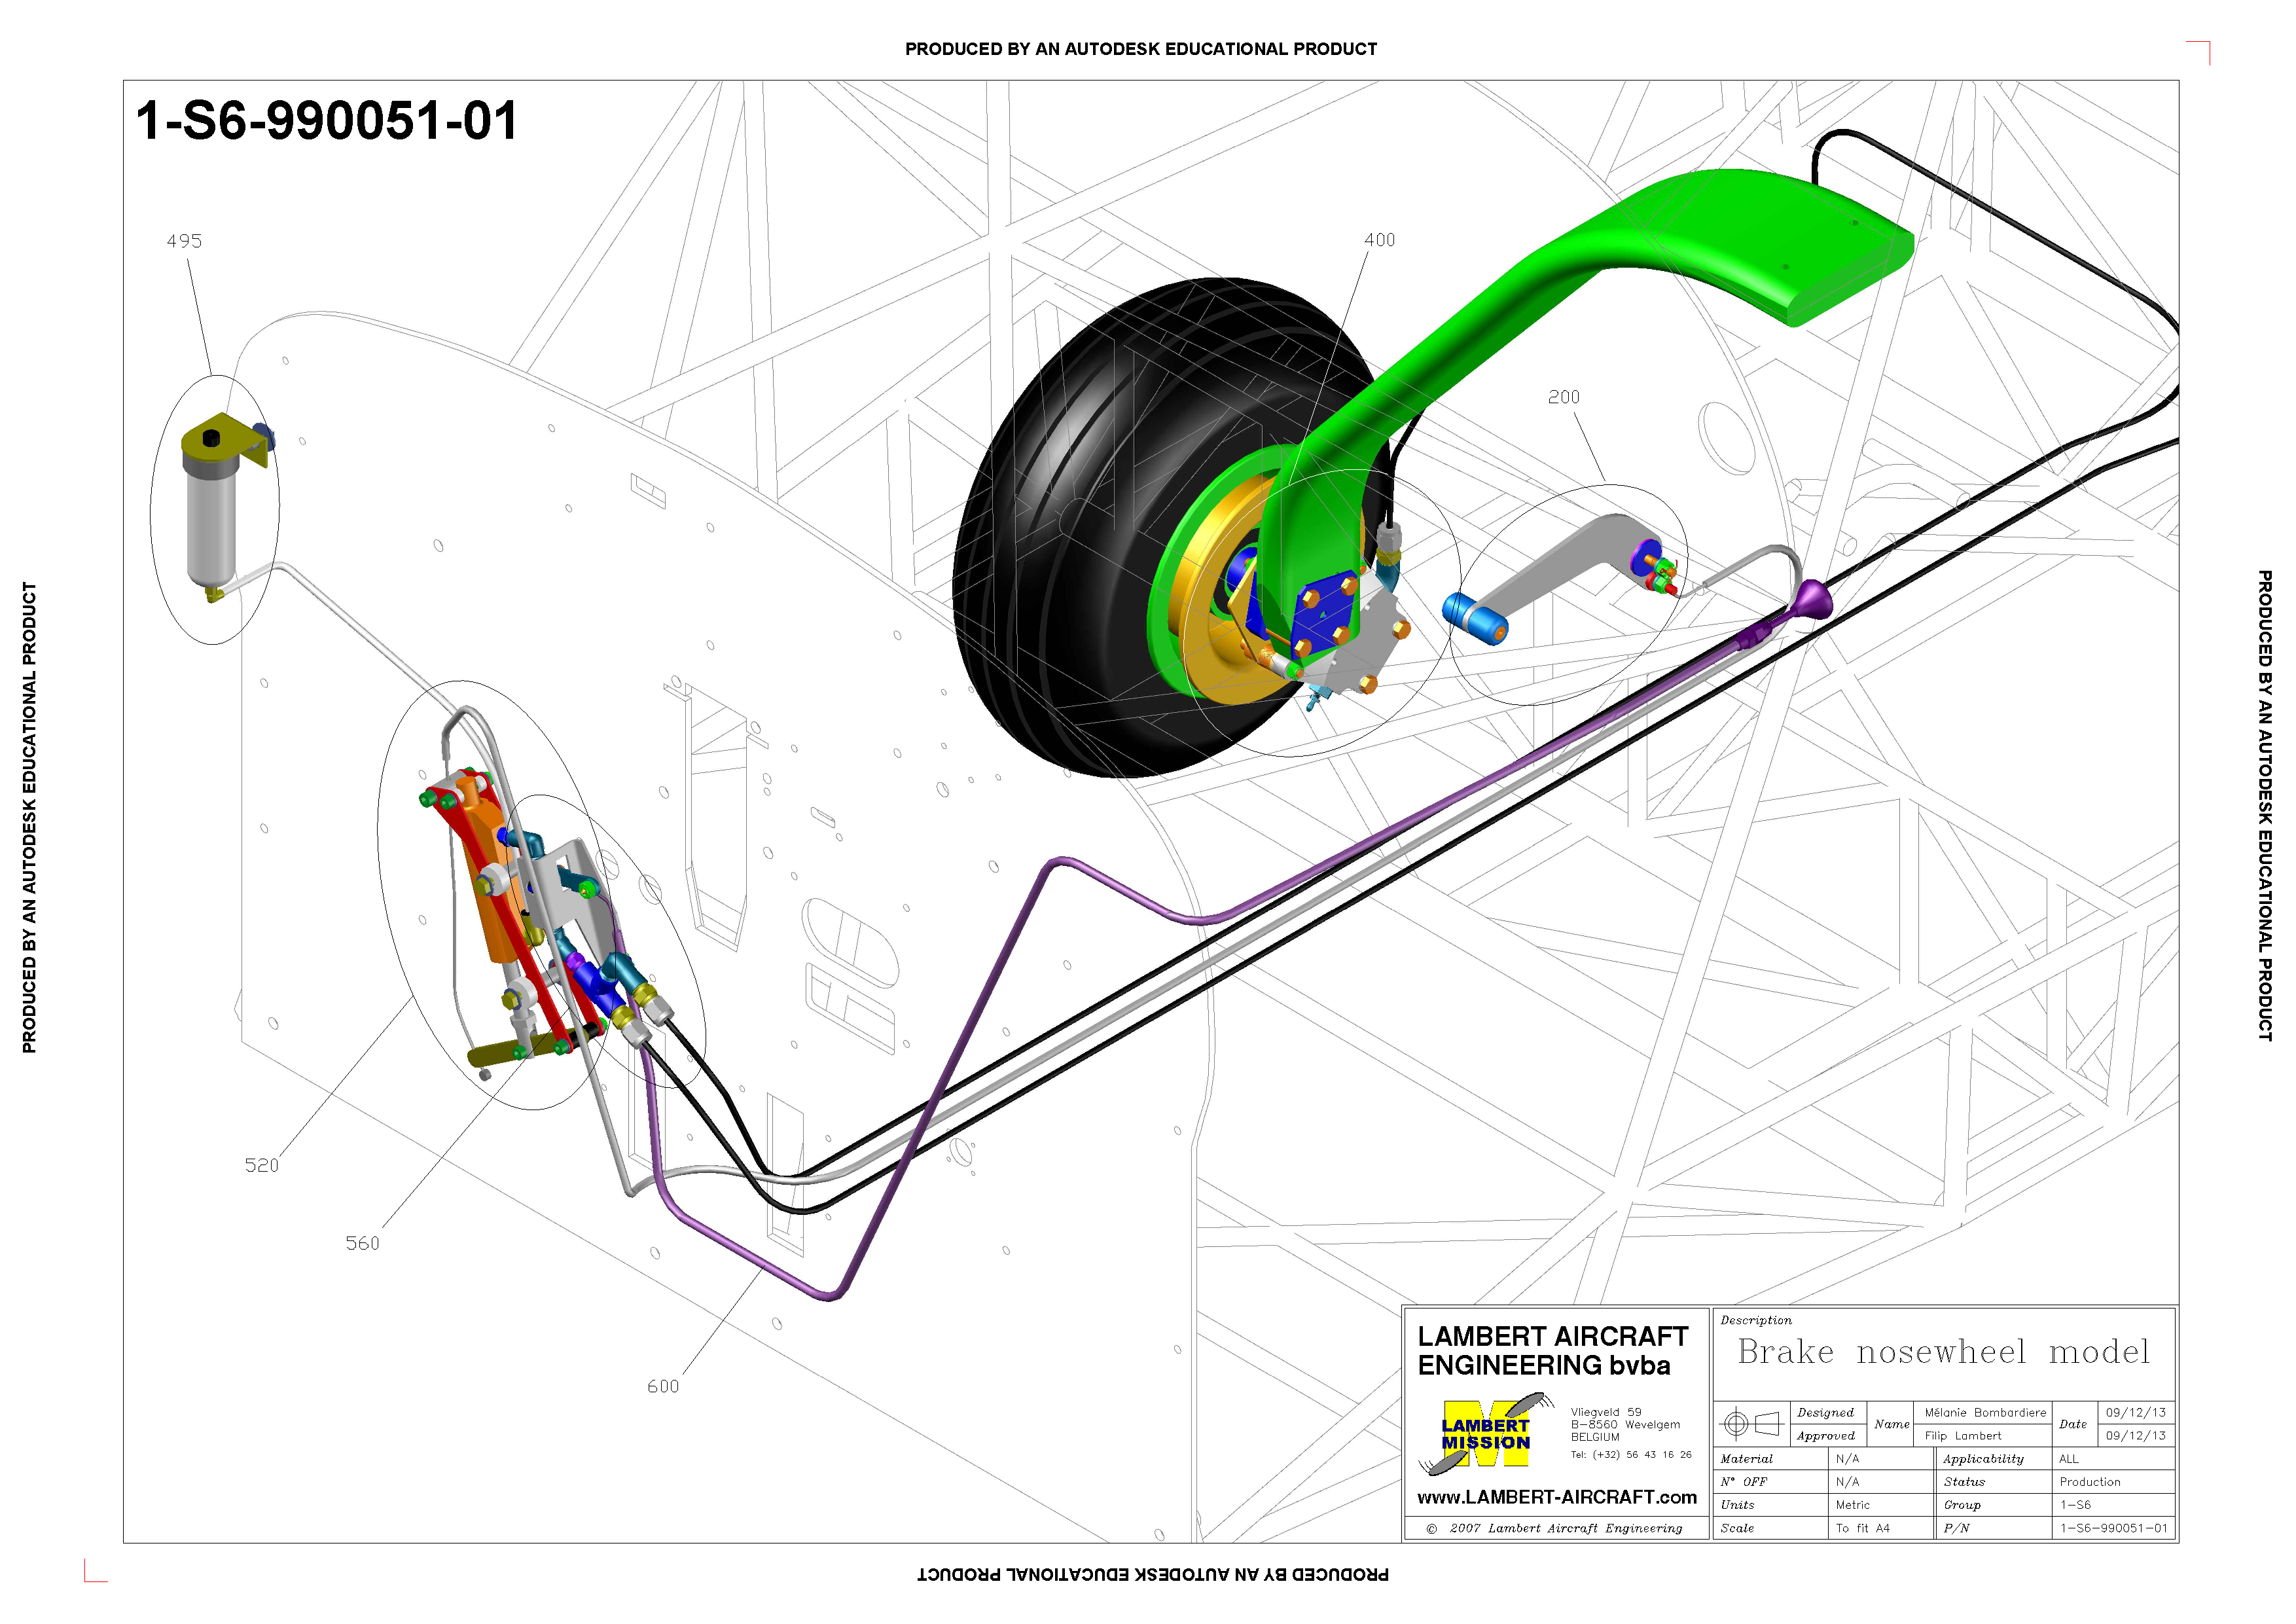
\includegraphics[width=15cm,trim = 1.5cm 2cm 1.5cm 2cm, clip]{pics/PIC023.pdf}
		\caption{The revised brake system}
		\label{fig:PIC023}
	\end{center}
\end{figure}


%TODO: refer to 2D drawings and partslist in annexe

\newpage

\subsection{Database}
LAMS (Lambert Aircraft Management System) is a new database recently created and still updated which will be used by the company. It will reference every part of the aircrafts by the part number.
%TODO: refer to the glossary section for the part number
I was assigned to test this experimental database in order to check the user interface for mistakes and improve it.

\subsubsection{Description of the database}
The database has been programmed in coordination with a computer engineer in order to obtain the following structure:
\begin{itemize}
\setlength{\itemsep}{0pt}
\item the airplane: Mission M108 or Mission M212;
\item the group: fuselage, cabin heating system etc;
\item the full assembly of the group;
\item the assembly;
\item the sub-assembly;
\item the nature of the part: 
\begin{itemize}
\setlength{\itemsep}{0pt}
\item part available for sale;
\item part of a welded structure (embedded part). It is available for the production but then, it is not possible to order it separately;
\item unfinished part, for example a part which needs to be bent (in-process part).
\end{itemize}

\end{itemize}
%TODO: structure of the database PIC024
\begin{figure}[ht!]
	\begin{center}
		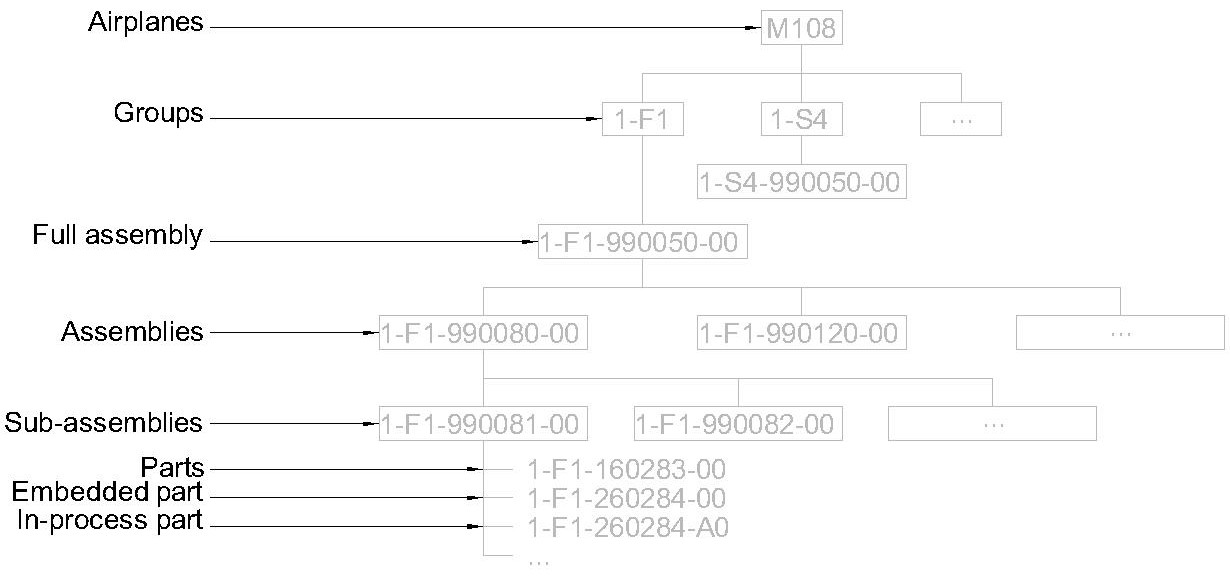
\includegraphics[width=15cm]{pics/PIC024.jpg}
		\caption{The database structure}
		\label{fig:PIC024}
	\end{center}
\end{figure}

\begin{fullpar}
Each part is described thanks to its part number but also to its status. The status can be one of this five following possibilities:
\begin{itemize}
\setlength{\itemsep}{0pt}
\item provisional: the part is not cleared yet for production, development only;
\item production: the part is used in the current production of the aircraft;
\item discontinued: the part is no longer installed in production, but is still available as a spare part for previous aircrafts;
\item obsolete: the installation of the part is permitted, but is no longer available;
\item withdrawn: the installation of the part is not permitted.
\end {itemize}
\end{fullpar}

Parts which are not produced by the company are also in the database. In this case, they have their internal part number and their serial number from the supplier. They are ready to be ordered. For instance, avionics instruments like transponders, radios and autopilots are referenced in the database.

\bigskip

We chose to test the database with the 1-S6 section (brake system). The parts list is quite complete and is not yet to be scheduled for any change. We also have different kinds of parts in this section and a little design change, we thus have two revisions. The brake system seemed to be the best section to have some experiments with the database.

\bigskip

%TODO: structure of the brake system assembly PIC025
\begin{figure}[ht!]
	\begin{center}
		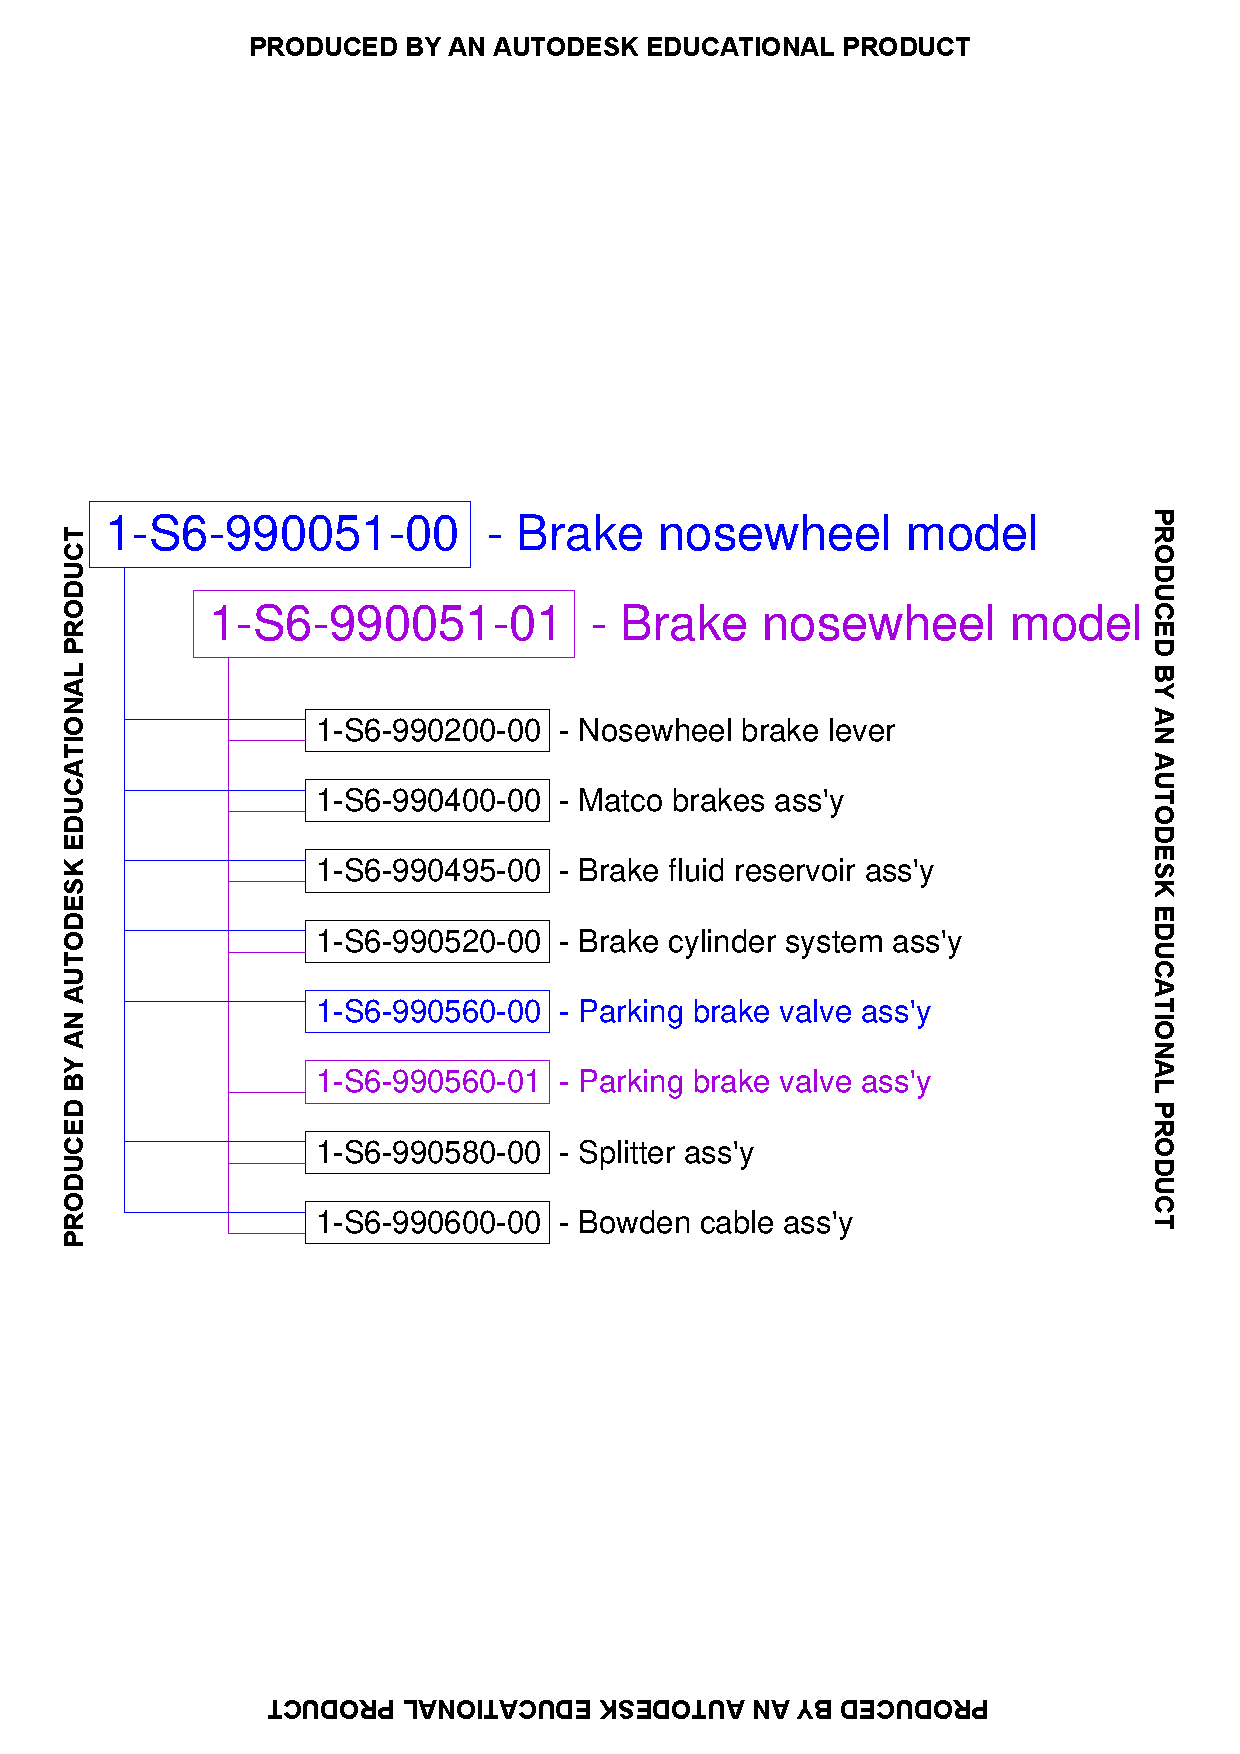
\includegraphics[width=10cm,trim = 1.5cm 8.5cm 1.5cm 8.5cm, clip]{pics/PIC025.pdf}
		\caption{The brake system structure}
		\label{fig:PIC025}
	\end{center}
\end{figure}

\newpage

\subsubsection{What it needed to be improved}
Some little problems have been noticed like too short strings sometimes for the description of the part (status, material...).
Certain issues were raised while we were adding new parts. The most important one is the LSTC structure: how can we have a logical structure for an assembly but also with the embedded LSTC's we can have? %refer to glossary and the 1-S2 structure

\bigskip

We need to be able to find easily ALL the parts needed for a LSTC. For example, if we take the example of the LSTC 1-007 (which corresponds to the optional cabin heating system for the M108 aircraft), we should be able to know what parts we have in stock or if we need to order some of them and what parts we need to make ourselves.
This should also be available for embedded LSTC's: for instance, LSTC's 1-014 to 1-017 (which correspond to the radio, transponder, com and autopilot installation) are only available for LSTC 1-013 (which corresponds to the TL panel).

%TODO: present the design of interior panels for cabin and my future work on that

\newpage

\section{Results}
\subsection{Evaluation of my contribution}
 I was pleased to see that even though I was an intern, I was assigned tasks that give a valuable contribution to the company. When my internship ended, almost all the documents and projects I had to work on were implemented and functional. The unfinished ones have been left with instructions in order to know what remains to be done. The main cause is the delay of receiving parts or documents which have postponed some projects.

\subsection{Technical knowledge acquired}
This was also an opportunity for me to acquire some knowledge on a large panel of technologies and methods of production in the aeronautical field. For instance, how an aircraft works:
\begin{itemize}
\setlength{\itemsep}{0pt}
\item on the mechanical aspect
\begin{itemize}
\setlength{\itemsep}{0pt}
\item the fuel system
\item the Rotax 912iS engine installation
\item the enginecooling and oil-cooling systems
\item the trim tab control
\item but also the different ways of production
\end{itemize}
\item on the electrical aspect
\begin{itemize}
\setlength{\itemsep}{0pt}
\item Engine Control Unit (ECU)
\item autopilots: pitch and roll servos
\item avionics shelf
\end{itemize}
\end{itemize}

\subsection{Human experience acquired}
Exchanging information is essential to get a project finished on time. 

\bigskip

Following up every little thing in one department was easy because we are in a same office but with other departments, sharing information was necessary. I quickly got used to this way of working because we were a few employees and information flows very quickly.

\bigskip

We were in constant communication with the customer to satisfy the best his expectations and adapt our ideas. Prototyping parts with a sheet of paper seems sometimes old-fashioned and eco-unfriendly but this is the best way to explain and show our suggestions.

\newpage

\section{Conclusion}
Lambert Aircraft Engineering is specialized in limited series production of aircrafts and in avionics maintenance. The objective of the internship was mainly to complete the documentation in parallel with the production of the first M108 with a new engine and in preparation of limited series production. I was part of the design team, following the production department in order to be aware of design changes and draw or update new parts for the aicraft.

\bigskip

The amount of tasks that were assigned to me, as well as their importance, was rewarding and made me feel valuable for the company. I worked on very challenging problems that deal with a large set of technologies, going from production drawings in 2D and 3D, database to design of the interior panels for the cabin. I worked closely with other engineers and technicians that were eager to assist and help me with any concern I had.

\bigskip

This internship confirmed my desire to specialize in aeronautical engineering but also developed my attraction to materials and welded structures. Working with talented, experienced engineers gave me a good understanding of what is to be expected for an engineer. The qualities that stroke me the most are: passion for aviation, willingness to leverage existing products and tools, being able to take decisions quickly, trying new technologies, and more generally getting things done!

\bigskip

I would like to thank Filip and Steven Lambert for giving me the opportunity to work on such an amazing project. I also would like to give a special thanks to Brecht Declerck for taking the time every day to help me and answering all my questions during those four months. Finally, I want to express my gratitude to all the members of the company for giving me some of their time, trusting me and letting me work in a very nice and friendly environment. It was a pleasure working with all of you.

\newpage

\section{Glossary} 
\subsection{LSA certifications}
\subsubsection{ASTM: American Society for Testing and Materials}
The Light Sport Aircraft (LSA) certification has been created by the ASTM in 2003 for aircrafts with these following characteristics:
\begin{itemize}
\item Maximal speed : 120 kt (222km/h)
\item Maximal weight: 600kg
\item Maximal stall speed : 45 kt (83km/h)
\item Single engine
\item Maximum 2 seats
\item Fixed landing gear
\item Fixed pitch or ground adjustable propeller
\item Non-pressurized cabin
\end{itemize}

\bigskip

Building aircrafts certified LSA as an amateur or professionnal is approved with the ASTM F-37 standard.

\subsubsection{EASA: European Agency for Safety Aviation}
The LSA standard from ASTM International is partially accepted by the EASA that refuses series production of light sport aircrafts in Europe. However, it allows amateurs to build one, under condition of being certified by the host country of the aircraft. This requires Lambert Aircraft Engineering to sell the Mission M108 LSA kit in Europe to homebuilders.

\subsubsection{FAA: Federal Aviation Administration}
The LSA standard from ASTM is totally accepted by the FAA and allows series and amateur production of light sport aircrafts. The core task of Lambert Aircraft Engineering is to produce M108 to the USA in series.

\subsubsection{STC's and LSTC's}
%LSTC =! STC (Supplemental Type Certificate)
A Supplemental Type Certificate is a modification which needs to be approved by the FAA even if the airplane has already been certified (without this major modification). A LSTC is specific to Lambert Aircraft Engineering company: it is a modification to the airplane which doesn't need the approval of the FAA but only an ``internal'' approval.

\bigskip

Actually, it is more used as an option for the aircrafts but sometimes, you have to choose between some LSTC. For example:
\begin{itemize}
\item If you want an instrument panel with the TL Elektronic main display, you will have to ask for LSTC 1-001 but if you want the Garmin G3X instrument panel, you will ask for LSTC 1-002. In any case, you have to choose between LSTC 1-001 or LSTC 1-002 because it is essential to have an instrument panel in your airplane!
\item However, if you want a cabin heating system (which is not essential to fly), you may ask for LSTC 1-007.
\end{itemize}

\subsubsection{Part classification system used in the company}
PART NUMBER (Aircraft, group, material code, part number, revision)
A part number is structured like the following template:
Aircraft - Group - Material code Number - Revision

Aircraft: ``1'' refers to the M108, ``2'' refers to the M212
Group: This can be a letter with a number referring to a system
Material: This is a number referring to a specific material
Number: This is the part number
Revision: This is a number which is incremented each time we have a new revision of the part.

%TODO: example

\subsubsection{Nosewheel and tailwheel models}

\begin{figure}[ht!]
	\begin{center}
		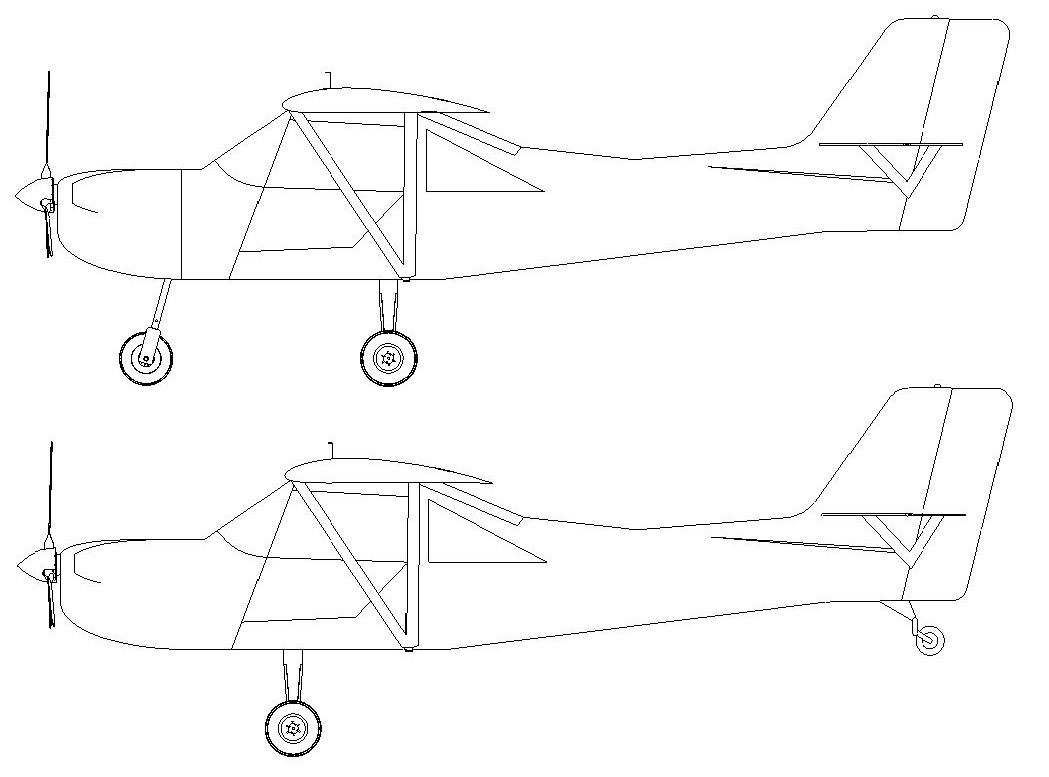
\includegraphics[width=10cm]{pics/PIC018.jpg}
		\caption{The nosewheel model (above) and the tailwheel model (under)}
		\label{fig:PIC018}
	\end{center}
\end{figure}

%TODO: explain how the tailwheel version works. 
%LANDING GEARS AND BRAKES RUDDER PEDALS

\end{document}
